\section{The effect of motion within frames}
\label{sec:res_beams_motion}
Going past the assumption of static scenery within frames, the experiments of this section aim to provide an understanding of the possible effects of motion within frames and the limitations resulting from it.
Adaptive beamformers are generally based on models assuming multiple static uncorrelated reflectors in the imaged medium. Section \ref{sec:spatial_smoothing} focused on divergences from the model due to the highly correlated nature of the reflected signals. Moving reflectors are also diverging from the assumed model, which might result in visible artifacts.

In Section \ref{sec:res_frames_motion}, the experiments focused on scatterer points moving at the array focus radius, since it was assessed to be the motion type causing the highest scalloping loss.
This motion type occurs very rarely, if ever, in real ultrasound imaging. This section focuses on more realistic scenarios with various linear motion types.

In this section, the velocity $\boldsymbol{v}_s$ of a scatterer point $s$ is defined as  $\boldsymbol{v}_s = (v_x, v_y)~$m/s, where the X axis is the image azimuth dimension and Y its range dimension. An illustration of a beamformed image with various examples of linear motion directions $\boldsymbol{v}_s$ at $10~$m/s is displayed in Figure \ref{fig:velocities}.
Within a single frame, motion is simulated by shifting a scatterer point before every beam transmit. Let us for example consider a scatterer point located $40~$mm from the array and moving laterally at $\boldsymbol{v}_s = (5, 0)$ m/s. With a single beam transmit taking 0.2 ms, the scatterer point is laterally shifted $5~$m/s$~\cdot~0.2~$ms $= 1~$mm per transmit beam.

It is of interest to compare $\boldsymbol{v}_s$ to the image acquisition time $t_{im}$, since a long image acquisition time is expected to result in higher sensitivity to scatterer points motion.
Equation (\ref{eq:acquisition_time}) defined the image acquisition time as function of the number of transmit beams $b_{tr}$. 
In this thesis, the simulated probe always transmits beams sequentially from left to right (towards positive X). 
In order to relate the scatterer points velocity $\boldsymbol{v}_s$ to the acquisition time $t_{im}$, Equation (\ref{eq:vtr_init}) defines the transmit beams distribution lateral velocity $v_{tr}$ as:
\begin{equation}
    v_{tr} = b_{tr} \cdot d_b / t_{im},
\label{eq:vtr_init}
\end{equation}
\noindent
where $d_b$, defined in Equation (\ref{eq:dist_beams}), is the lateral distance between two beams at range $r$. Combining Equations (\ref{eq:acquisition_time}) and (\ref{eq:dist_beams}), Equation (\ref{eq:vtr_init}) becomes:
\begin{equation}
    v_{tr} = \frac{b_{tr} \cdot 0.3 \cdot r \cdot c}{2 \cdot \lfloor b_{tr} / 2 \rfloor \cdot r_{max} \cdot b_{tr}} = \frac{1500 \cdot r}{\lfloor b_{tr} / 2 \rfloor},
\label{eq:vtr}
\end{equation}
where $r_{max} = 0.15~$m is the maximum acquisition radius, $c = 1500~$m/s the transmitted signals' speed of propagation and $\lfloor \rfloor$ is the floor operator. 
For example, let us imagine an image illuminated by $b_{tr} = 11$ transmit beams. Their lateral velocity at $40~$mm range is $v_{tr_{40}} = 1500 \cdot 40 \cdot 10^{-3} / 5 = 12~$m/s, and at $55~$mm range $v_{tr_{55}} = 1500 \cdot 55 \cdot 10^{-3} / 5 = 16.5~$m/s. This example is illustrated in Figure \ref{fig:velocities}.
\begin{figure}[ht]
    \centering
    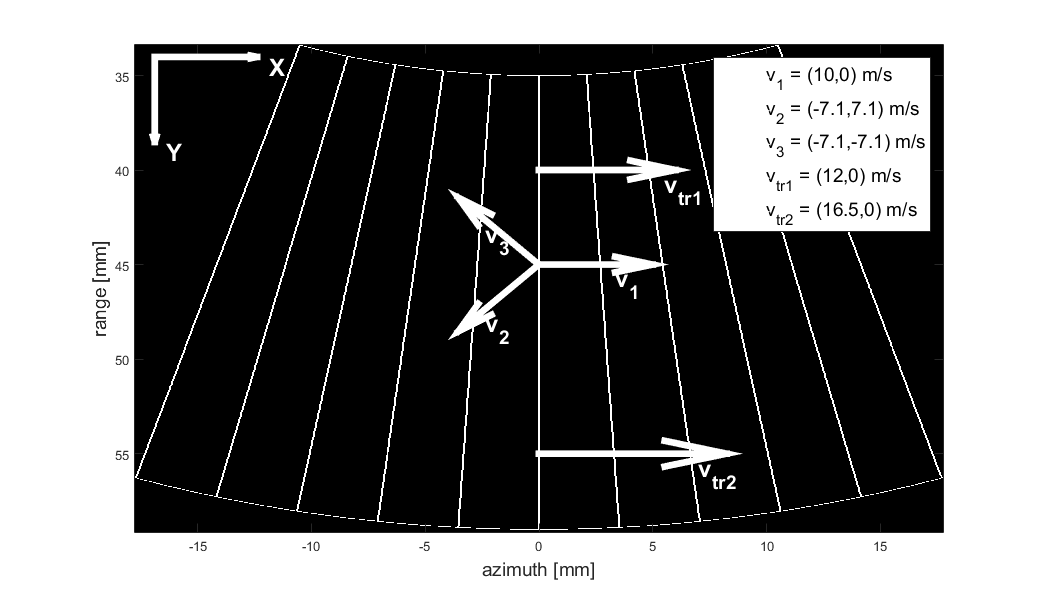
\includegraphics[width=\linewidth]{./images/results/2.1/velocities.png}
    \caption[Illustration of beamformed image with various velocities.]{Illustration of beamformed image with various velocities. The velocity vectors are at a different scale than the image azimuth and range.}
    \label{fig:velocities}
\end{figure}

If not mentioned otherwise, all beamformed images of this section are considered to be built from $b_{tr} = 65$ transmit beams and $b_{re} = 3 \cdot 65 = 195$ receive beams. The number of transmit beams corresponds to the required number of beams to guarantee no visible scalloping loss for DAS in a noiseless medium and $b_{re} = 195$ ensures no visible scalloping loss for the IAA and DAS beamformers (Table \ref{table:num_beams}).
In order to simulate perfect multiline acquisition (MLA) on reception, the images are actually created from $b_{tr} = b_{re} = 195$ beams, but the image acquisition time is still considered to be $t_{im} = 0.3 \cdot 65 / 1500 = 0.013~$s = 13 ms.
We could also have chosen $b_{re} \geq 981$ in order to ensure no visible scalloping loss for the MV beamformer as well, but 
such high beam densities are too computationally demanding for us to run all the experiments with such simulations.
Furthermore, we consider such beam densities to be too high to be realistically implementable and therefore not very interesting to analyze.

The linear motion of a scatterer point is, as explained previously, simulated with a constant shift of its position before each beam transmit and recording. With the MLA approach, the scatterer points should actually only move in between two transmit beams and remain static for receive beams constructed from the same transmit beam. With a MLA coefficient of $MLA_c = b_{re} / b_{tr} = 195 / 65 = 3$, the scatterer points should only be shifted once every three receive beams.
We have however chosen to have the scatterer point shifted in between all beams for two main reasons.
First of all, with continuous motion, the results of this section can be extended to MLA approaches with virtually any coefficient value $MLA_c$, including single-line acquisition ($MLA_c = 1$). Secondly, this thesis focuses on worst-case scenarios and continuous motion seems to us to be a bigger divergence from the beamformers' model of static points than partial motion. We do not expect the partial motion implementation to result in additional artifacts.


\subsection{Single scatterer point in a noiseless medium}
\label{sec:single_noiseless}
In this thesis, a scatterer point shape in a beamformed image is defined by the area within 3 dB of its peak gain. This section focuses on imaging a single scatterer point and analyzing the effects of motion within frames on its shape.

As initial exposure to motion within frames, let us start with a simple example. A single scatterer point $s$ is positioned at $40~$mm range and $0~$mm azimuth in a noiseless medium. In this example, $s_1$ is imaged with different lateral velocities $\boldsymbol{v}_s = (v_x, 0),~ v_x \in \{-0.6, 0, 0.6\}~$m/s.
The DAS beamformed image and steered response of $s_1$ when static are displayed in Figure \ref{fig:DAS_steered}. The problems with those plots are that the beamformed image does not clearly outline the shape of the scatterer point and the steered response plot only shows its width. Instead, we have chosen to replace both plots with a contour plot of the beamformed image with 3 color-coded gain levels (from darkest to brightest): max-100, max-10 and max-3 dB.
Figure \ref{fig:DAS_steered} can then be replaced by the DAS contour plot of Figure \ref{fig:DAS_idle}, where the white area represents the perceived shape of the scatterer point.
This contour plot representation is used as a visualization tool for the rest of this thesis.

\begin{figure}[ht]
    \centering
    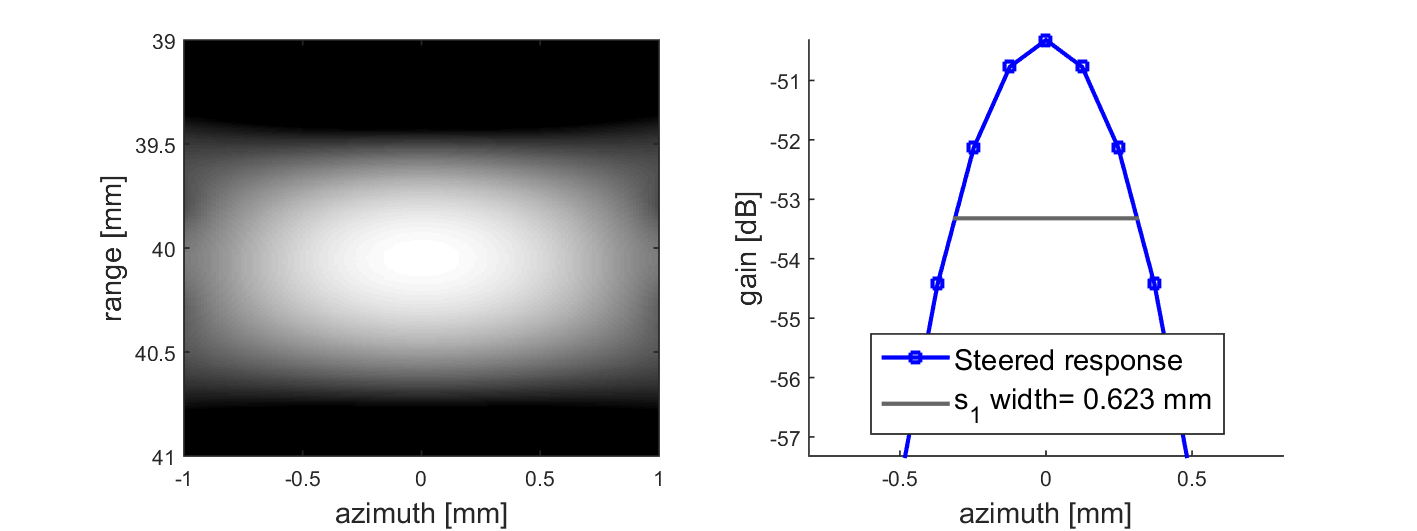
\includegraphics[width=\linewidth]{./images/results/2.1/DAS_steered2.png}
	\caption{DAS beamformed image and steered response of a static scatter point in a noiseless medium.}
	\label{fig:DAS_steered}
\end{figure}

\begin{figure}[ht]
    \centering
    \begin{subfigure}[t]{0.48\linewidth}
        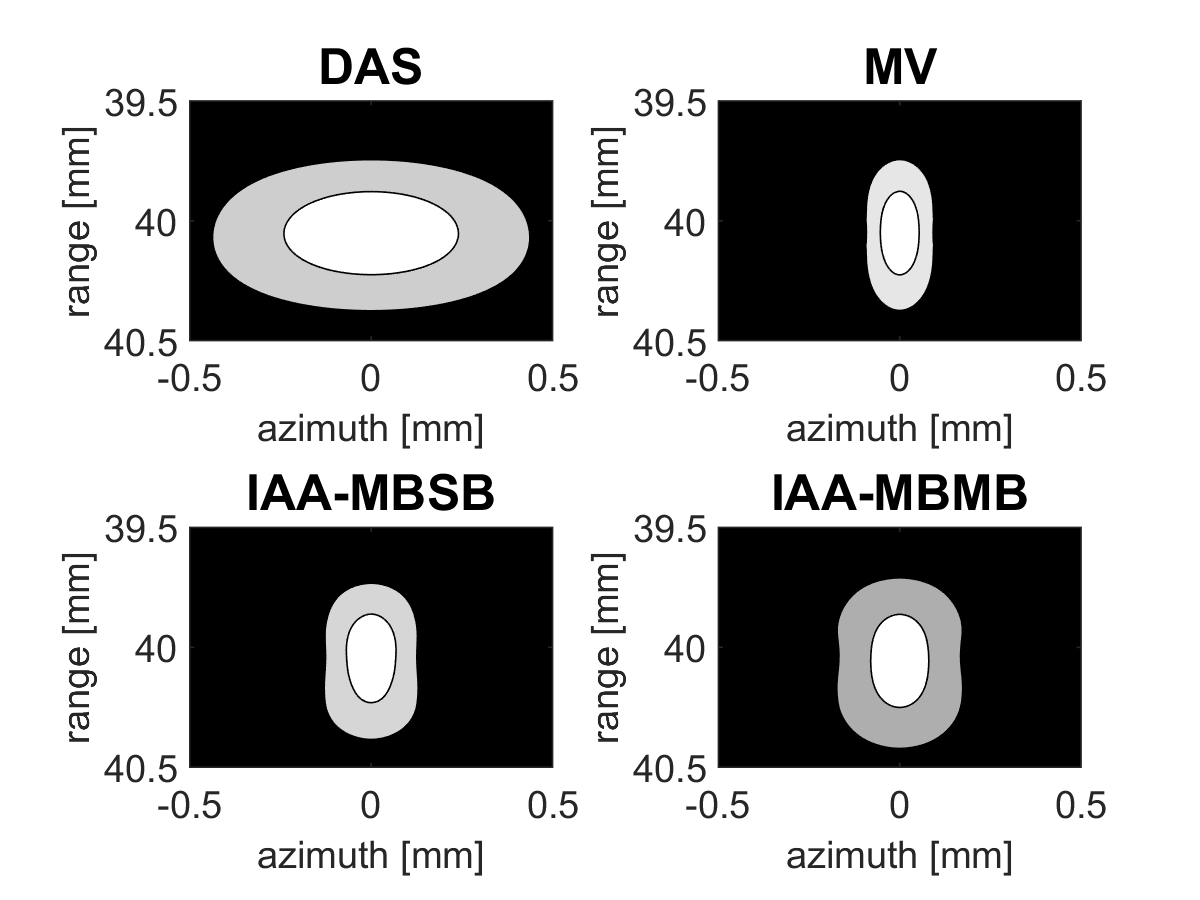
\includegraphics[width=\linewidth]{./images/results/2.1/motion_0_-06.png}
        \caption{$v_x = -0.6~$m/s.}
    \end{subfigure}
    \quad
    \begin{subfigure}[t]{0.48\linewidth}
        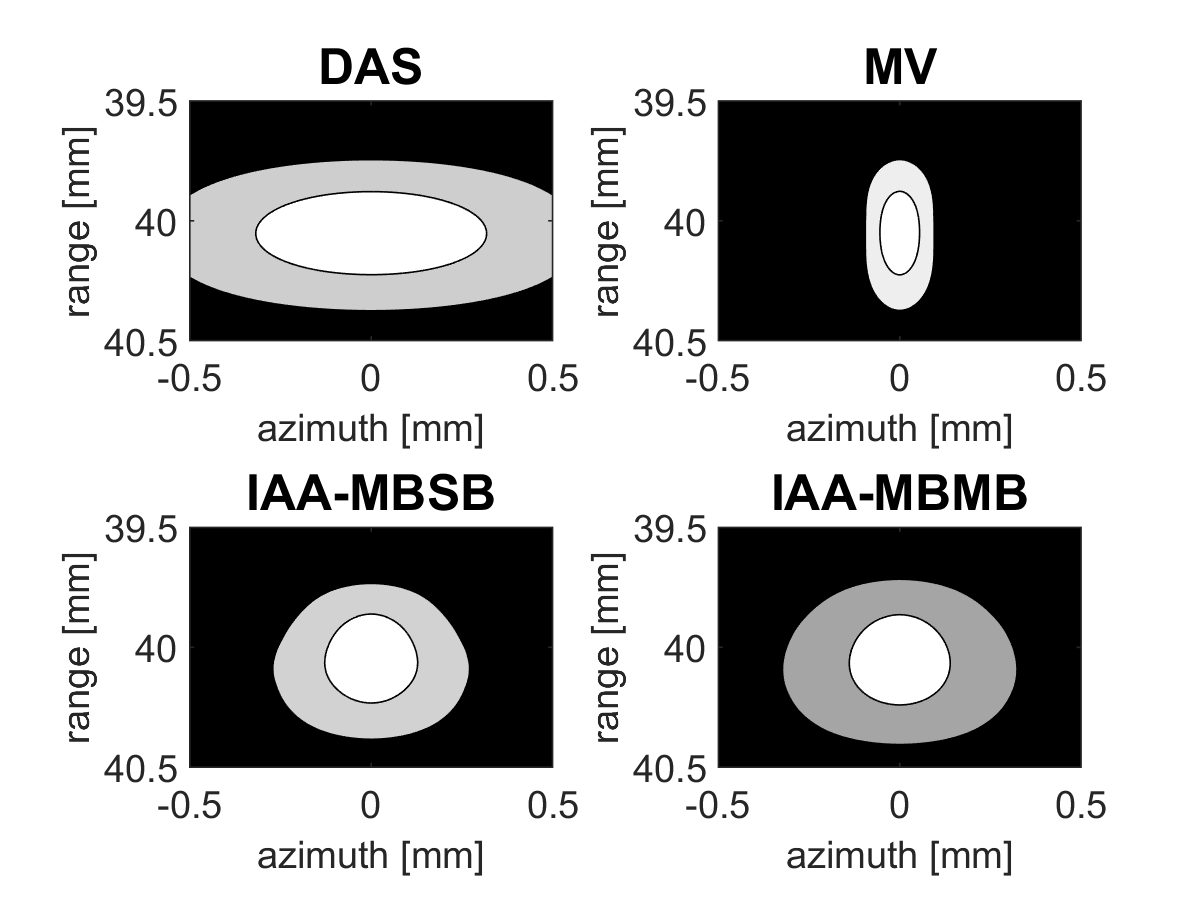
\includegraphics[width=\linewidth]{./images/results/2.1/motion_0_0.png}
        \caption{$v_x = 0~$m/s.}
        \label{fig:DAS_idle}
    \end{subfigure}
    \quad
    \begin{subfigure}[t]{0.48\linewidth}
        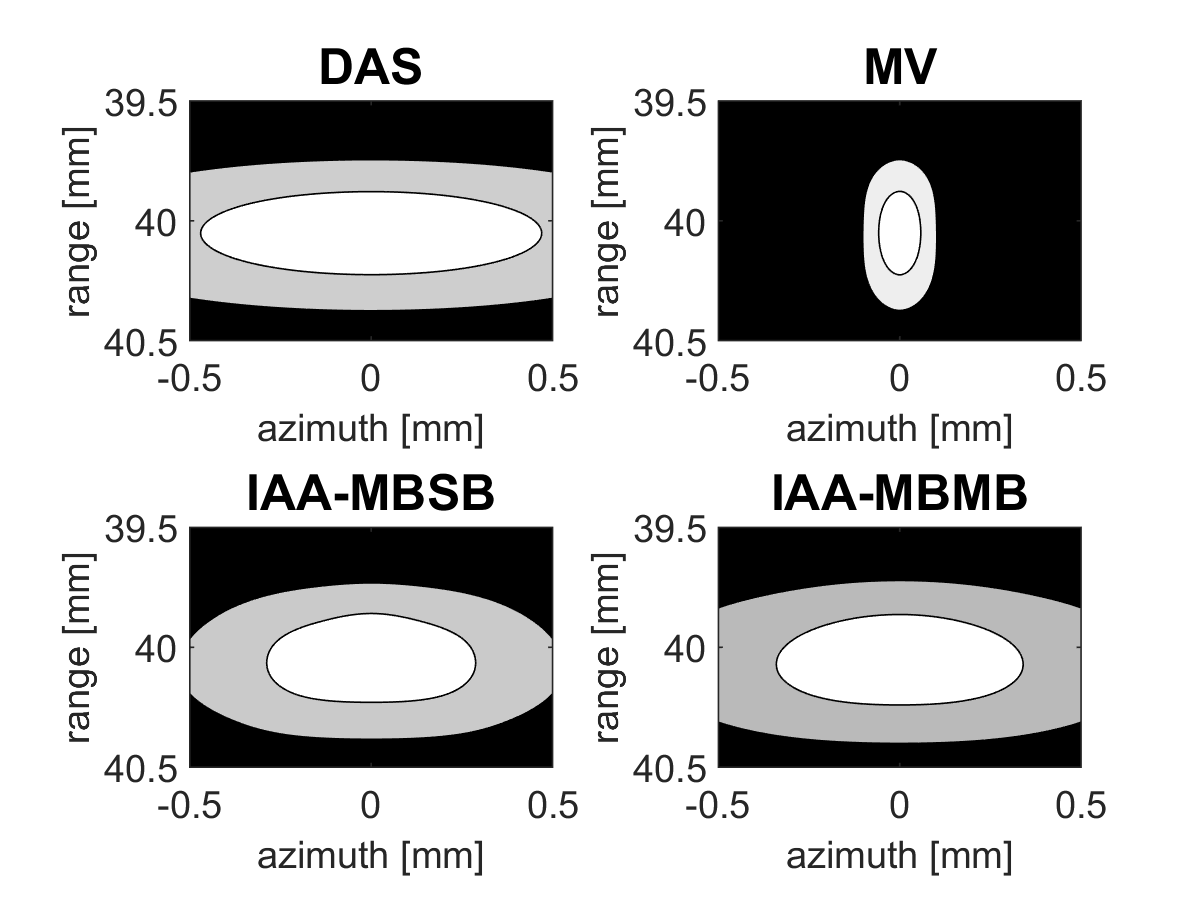
\includegraphics[width=\linewidth]{./images/results/2.1/motion_0_06.png}
        \caption{$v_x = 0.6~$m/s.}
    \end{subfigure}
	\caption{Contour plot of DAS beamformed images. Scatter point in lateral motion in a noiseless medium: $\boldsymbol{v}_s = (v_x, 0)~$m/s, $v_x \in \{-0.6, 0, 0.6\}$.}
	\label{fig:illustration_all}
\end{figure}

Figure \ref{fig:illustration_all} displays the results of the current experiment for the three different velocities $v_x \in \{-0.6, 0, 0.6\}~$m/s and all beamformers.
First of all, the beamformers obviously have different resolution capacities, which is why the shape of the scatterer point varies so much depending on the beamformer used even if static (Figure \ref{fig:DAS_idle}). The comparison of the DAS and MV beamformed images gives a good example of why the MV beamformer has historically been introduced as a high-resolution algorithm.

Compared to the static scene, the scatterer point consistently appears bigger when it is moving in the same direction as $v_{tr}$ ($v_x > 0$) and smaller when $v_x < 0$, although the size variation is hardly visible in the MV beamformed images. The MV beamformer seems much less sensitive to lateral motion than the other beamformers.
But, besides this lateral dilation or erosion of the scatterer point's shape, none of the beamformed images seem to contain visible artifacts.
It is worth mentioning that, in this section, all images are built such that the scatterer point is at $0~$mm azimuth when the center beam is transmitted, regardless of the point's velocity, which is why the center of its shape always is at $0~$mm azimuth and $40~$mm range.
That way we limit potential artifact due to differences in the scatterer point's position, including possibly visible scalloping loss for the MV beamformer.
Note that a scatterer point having a linear motion type, even at constant range, has a varying radius to the array, which means that it can potentially go in and out of the array's focus radius.

For the next experiment, multiple frames are simulated with a single scatterer point located at $40~$mm range and moving at different lateral velocities $v_x$ from -0.6 to 0.6 m/s.
For any given frame, the width of the scatterer point is estimated by the mainlobe width of the array's steered response at $40~$mm radius. For each frame, the resulting scatterer point width is displayed in Figure \ref{fig:width_vs_velocity} both as an absolute value and as a relative increase, in $\%$, compared to that of the scatterer point when static.

\begin{figure}[ht]
    \centering
    \begin{subfigure}[t]{\linewidth}
        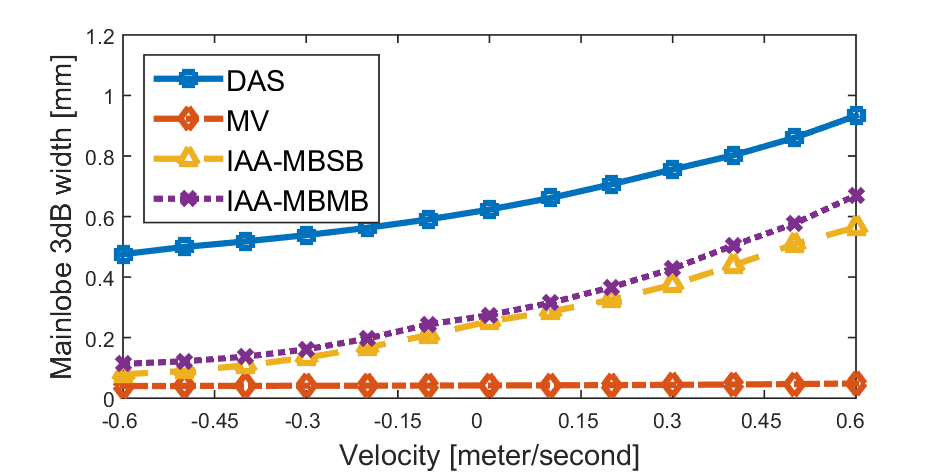
\includegraphics[width=\linewidth]{./images/results/2.1/mainlobe_width_65.png}
        \caption{Steered response mainlobe width in mm.}
        \label{fig:width_vs_velocity_a}
    \end{subfigure}
    \quad
    \begin{subfigure}[t]{\linewidth}
        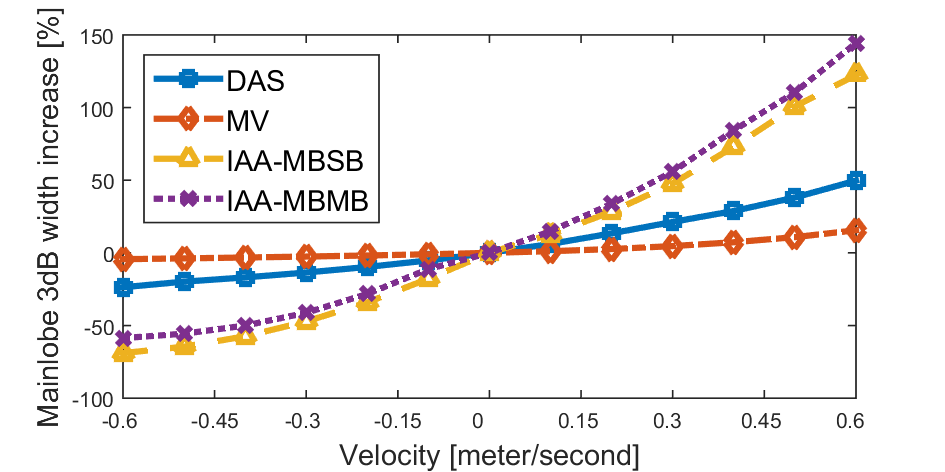
\includegraphics[width=\linewidth]{./images/results/2.1/mainlobe_width_65_rel.png}
        \caption{Steered response mainlobe width relative to that of the static scatterer point scenario.}
        \label{fig:width_vs_velocity_b}
    \end{subfigure}
	\caption{Scatter point in lateral motion in a noiseless medium: $\boldsymbol{v}_s = (v_x, 0)~$m/s, $-0.6 \leq v_x \leq 0.6$.}
	\label{fig:width_vs_velocity}
\end{figure}

As predicted in Table \ref{table:panoramic_imperfect}, the point's apparent width gets dilated with positive velocities along its motion path. Motions opposite to the beam distribution direction ($v_x < 0$) result in the point's width appearing smaller. This can be explained by the fact that the scatterer point potentially hits more transmit beams as $v_x$ increases. Following that principle, if $v_x$ increases to very high values, the apparent width of the scatterer point should decrease. The maximum apparent width should happen when $v_x$ is equal to $v_{tr}$, where $v_{tr}$ is defined by Equation (\ref{eq:vtr}). This statement can be confirmed by extending the current experiment to extreme velocities. The results with velocities $v_x \leq 3~$m/s are displayed in Figure \ref{fig:width_vs_velocity_ext_pos}. With $b_{tr} = 65$, the acquisition lateral velocity at $40~$mm radius is $v_{tr_{40}} = 1500 \cdot 40 \cdot 10^{-3} / \lfloor 65 / 2 \rfloor = 60 / 32 = 1.875~$m/s. For all beamformers, the scatterer point's width increases with its lateral velocity $v_x$ and peaks when $v_x = v_{tr}$, then decreases as $v_x$ increases beyond that. This effect is indeed not an artifact caused by a particular beamformer algorithm but by a physical limitation, even if different beamformers have different sensitivities to that effect.

\begin{figure}[ht]
    \centering
    \begin{subfigure}[t]{\linewidth}
        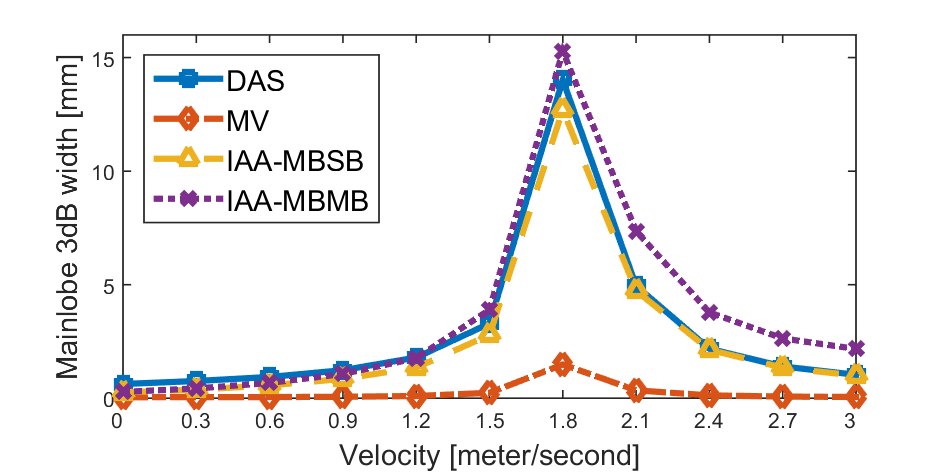
\includegraphics[width=\linewidth]{./images/results/2.1/speeds_ext_pos.png}
        \caption{$0 \leq v_x \leq 3~$m/s.}
	    \label{fig:width_vs_velocity_ext_pos}
    \end{subfigure}
    \quad
    \begin{subfigure}[t]{\linewidth}
        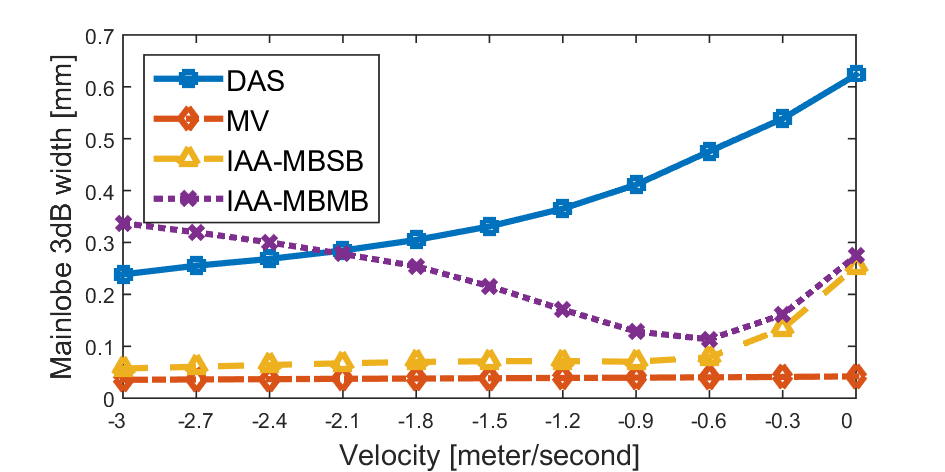
\includegraphics[width=\linewidth]{./images/results/2.1/speeds_ext_neg.png}
        \caption{$-3 \leq v_x \leq 0~$m/s.}
	    \label{fig:width_vs_velocity_ext_neg}
    \end{subfigure}
	\caption{Scatter point in lateral motion in a noiseless medium: $\boldsymbol{v}_s = (v_x, 0)~$m/s, $-3 \leq v_x \leq 3$.}
	\label{fig:width_vs_velocity_ext}
\end{figure}

In most imaging applications, one would want to avoid scenarios where $v_x$ converges towards $v_{tr}$, since the scatterer point can potentially appear much wider than it should and may result in a dramatic loss of resolution.
This imposes an upper limitation on the number of transmit beams. Such a limitation depends on how much resolution loss is considered acceptable, which depends on the application.
As an example, let us consider the limitation that any scatterer point should not move faster than 80\% of the beam distribution velocity: $v_x \leq 0.8 \cdot v_{tr}$.
Adding to that the assumption of Section \ref{sec:beams_motion} that $\boldsymbol{v}_s \leq 0.6$ m/s, the upper limit beam distribution velocity with this setup is: $v_{tr} = 0.6 / 0.8 = 0.75$ m/s. Since $v_{tr}$ is defined in Equation (\ref{eq:vtr}) as a function of the range $r$, for $b_{tr} = 65$, the upper limit of $v_{tr}$ implicitly sets a minimum range limit $r_{lim} = v_{tr} \cdot \lfloor b_{tr} / 2 \rfloor / 1500 = 0.75 \cdot 32 / 1500 = 16~$mm. This means that, in this example, resolution losses beyond what is considered acceptable might occur for range values $r < 16~$mm.

As mentioned previously, the cause of the apparent dilation or erosion of a scatterer point is a physical one, but different beamformers have different sensitivities to that effect. A quick comparison of the DAS and MV beamformers shows that the MV beamformer is much less sensitive to lateral motion, for the same beam density, both in terms of absolute mainlobe width or relative width increase. One could then speculate that, for singlebeam beamformers, their sensitivity to lateral motion is highly correlated with the mainlobe width of their receive beams.
Although we do not prove this speculation in this thesis, it seems logical that, given the same beam density, creating wider beams would result in the scatterer point hitting more of them and, consequently, lead to increased sensitivity to lateral motion.

Regardless of the veracity of this speculation, the sensitivity to lateral motion of the multibeam IAA approaches can not be solely explained from their mainlobe width. They appear indeed more sensitive to motion than their sheer mainlobe width would suggest.
The IAA beamformers are based on the sparse signal representation approach (\cite{Yardibi_nonparametric_IAA}), which means that they model static scatterer points and try to adapt that model to the recorded data.
A moving point does not fit well with this model since the different beams can potentially hold contradicting information about the presence of a scatterer point in a given direction.
When combining the receive beams into a multibeam covariance matrix estimate, the mismatch between the beams' information can cause distortions in the scatterer point's apparent shape.
We did not know how such a divergence between the expected model and the recorded data would affect the performance of the IAA beamformers.
We see from Figures \ref{fig:illustration_all} and \ref{fig:width_vs_velocity_ext} that this divergence only seems to result in loss of image resolution.
The IAA-MBSB beamformer is more sensitive than DAS in terms of relative loss of resolution, but still maintains an absolute resolution under or equal to that of the DAS.
The width of the scatterer point follows the same general pattern with the IAA-MBSB as with the singlebeam beamformers.
It increases with $v_x$, peaks at $v_x = v_{tr}$ and then decreases.

The IAA-MBMB, on the other hand, displays a different behaviour with $v_x \leq -0.6~$m/s. While, with the other beamformers, the width of the scatterer point diminishes with $v_x$ going towards $-\infty$, it appears with IAA-MBMB to grow back and even beyond its value when static.
The IAA-MBMB is also altogether more sensitive to lateral motion than IAA-MBSB and can yield results with lower resolution than DAS for relatively high velocities, both positive and negative.
Both the IAA-MBSB and IAA-MBMB beamformers suffer from this discrepancy of the imaged medium from the assumed model. However, the IAA-MBMB approach is more sensitive to this divergence since it uses the multibeam $\boldsymbol{\hat{R}}$ for the final estimate of the scatterer point amplitudes (Equation (\ref{eq:mb_output})), whereas the IAA-MBSB approach only uses the corresponding time- and phase-shifted array data for that final step (Equation (\ref{eq:sb_output})).

For the next experiment, scatterer points moving in different directions are imaged. The beamformed images are simulated in the same manner as for the previous experiment, with a single scatterer point moving in a noiseless medium. The only difference is that the scatterer point is not only assumed to move laterally ($v_x \neq 0$), but also vertically ($v_y \neq 0$). The goal of this experiment is to find out if the vertical component of a scatterer point's velocity induces additional artifacts in its apparent shape. Different scatterer point velocities $\boldsymbol{v}_s$  such that $|\boldsymbol{v}_s| = 0.6~$m/s are experimented with and the resulting beamformed images are displayed in Figure \ref{fig:linear_motion}.

The results of Figure \ref{fig:linear_motion} converge with those of Figure \ref{fig:width_vs_velocity} in the sense that motion within frames only seems to result in dilation or erosion of the scatterer point. However, it is worth noticing that the direction of dilation $\boldsymbol{d}_s = (d_x, d_y)~$m does not always correspond to the direction of motion $\boldsymbol{v}_s = (v_x, v_y)~$m/s. 
The Y component $d_y$ is always of same sign as $v_y$, but the X component is not only dependent on $v_x$, but also $v_y$ and $v_{tr}$.
Figures \ref{eq:vertical_towards} and \ref{eq:vertical_away} reveal that the scatterer point appears dilated along the X axis also with vertical linear motion ($v_x = 0$). 
Since the images are formed by sequentially transmitting beams from left to right ($v_{tr} \geq 0$), the direction of dilation has $d_x >0$ even if the scatterer point has no lateral motion. This can result in visual confusion of the direction of dilation, since the resulting scatterer point shape can look very much alike for various velocity directions.

\begin{figure}[ht]
    \centering
    \begin{subfigure}[t]{0.48\linewidth}
        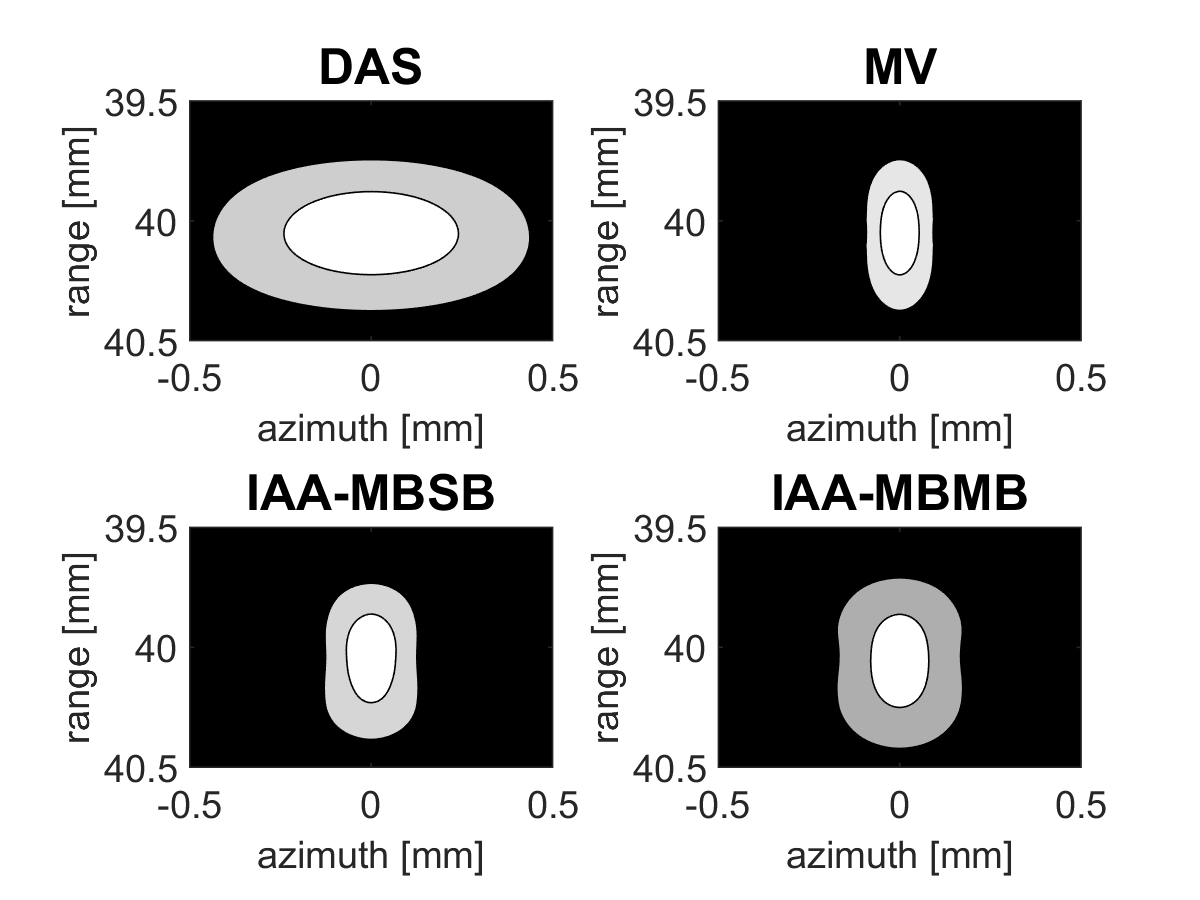
\includegraphics[width=\linewidth]{./images/results/2.1/motion_0_-06.png}
        \caption{$\boldsymbol{v}_s = (-0.6, 0)~m/s$.}
    \end{subfigure}
    \quad
    \begin{subfigure}[t]{0.48\linewidth}
        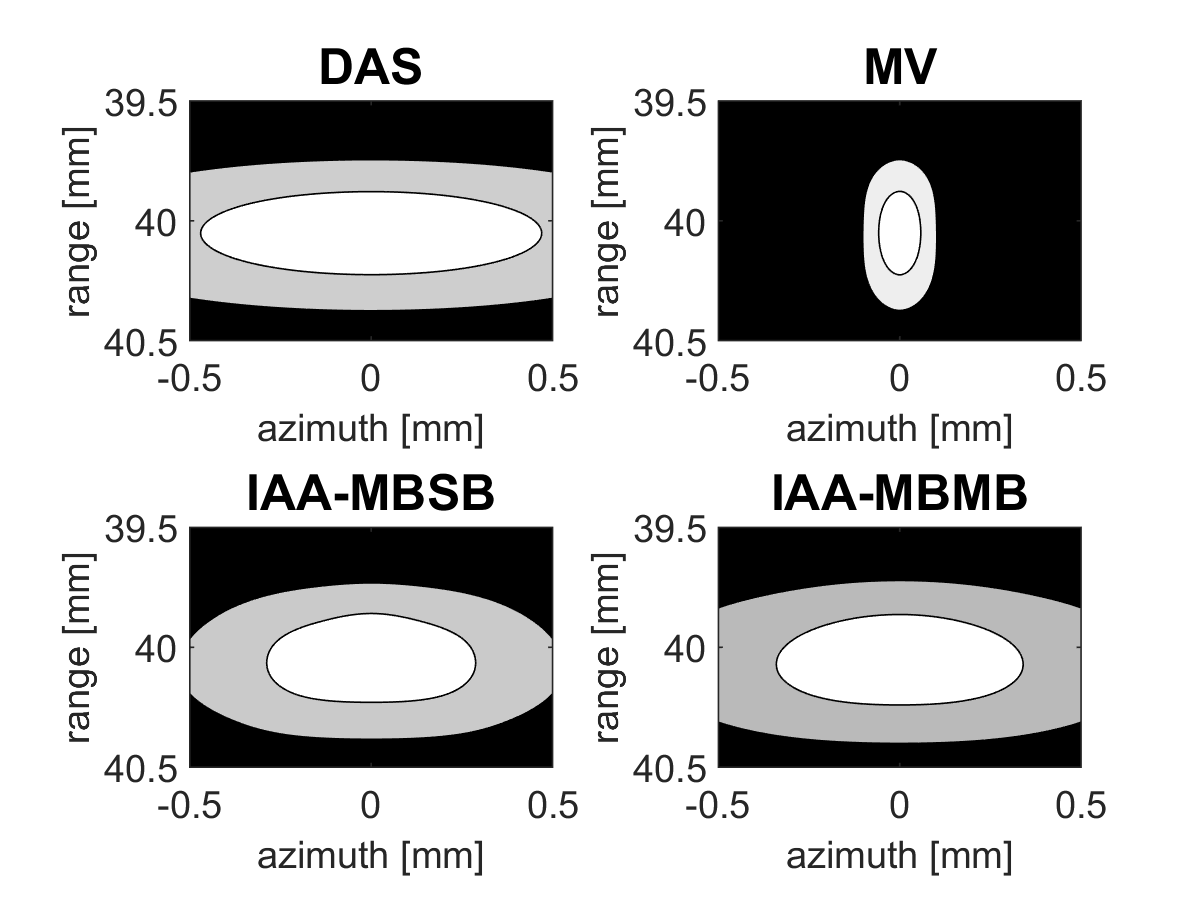
\includegraphics[width=\linewidth]{./images/results/2.1/motion_0_06.png}
        \caption{$\boldsymbol{v}_s = (0.6, 0)~m/s$.}
    \end{subfigure}
    \quad
    \begin{subfigure}[t]{0.48\linewidth}
        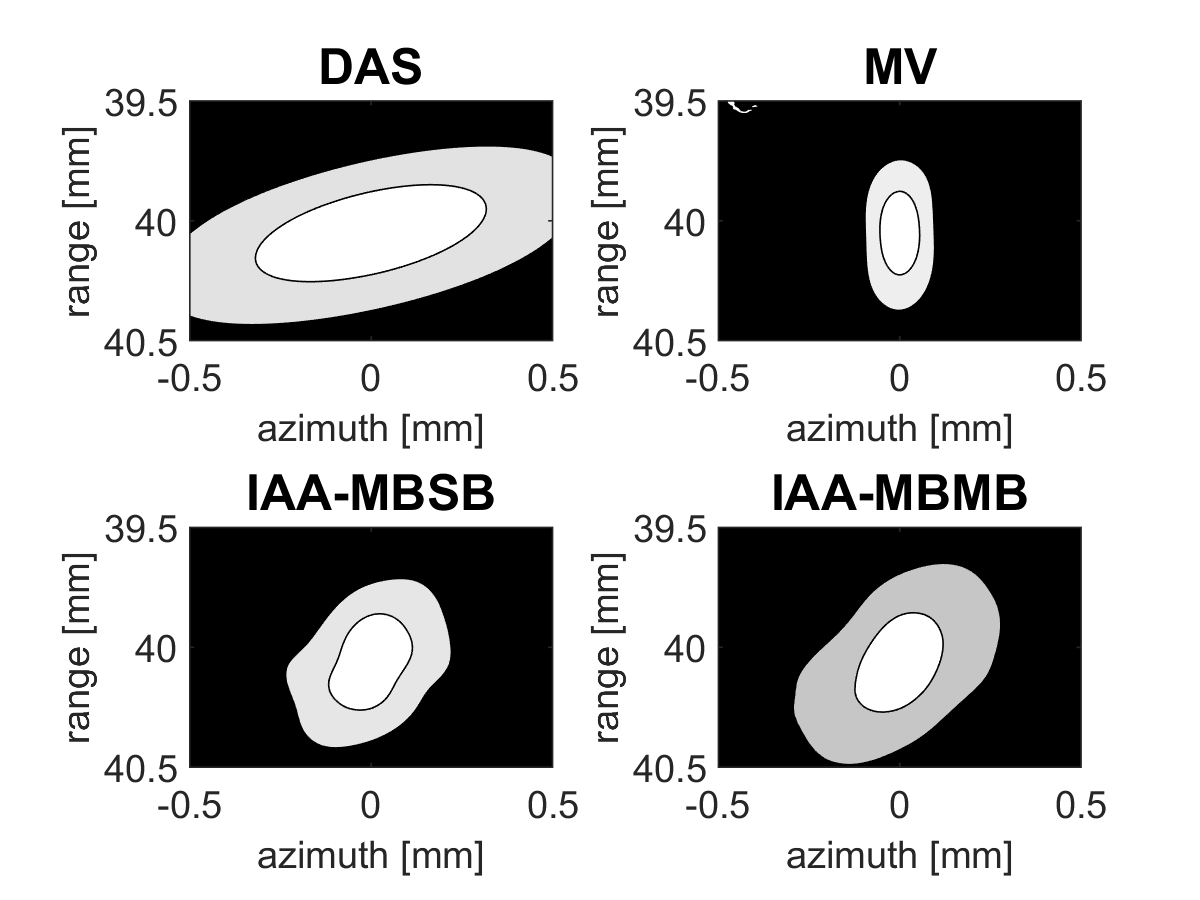
\includegraphics[width=\linewidth]{./images/results/2.1/motion_90_-06.png}
        \caption{$\boldsymbol{v}_s = (0, -0.6)~m/s$.}
        \label{eq:vertical_towards}
    \end{subfigure}
    \quad
    \begin{subfigure}[t]{0.48\linewidth}
        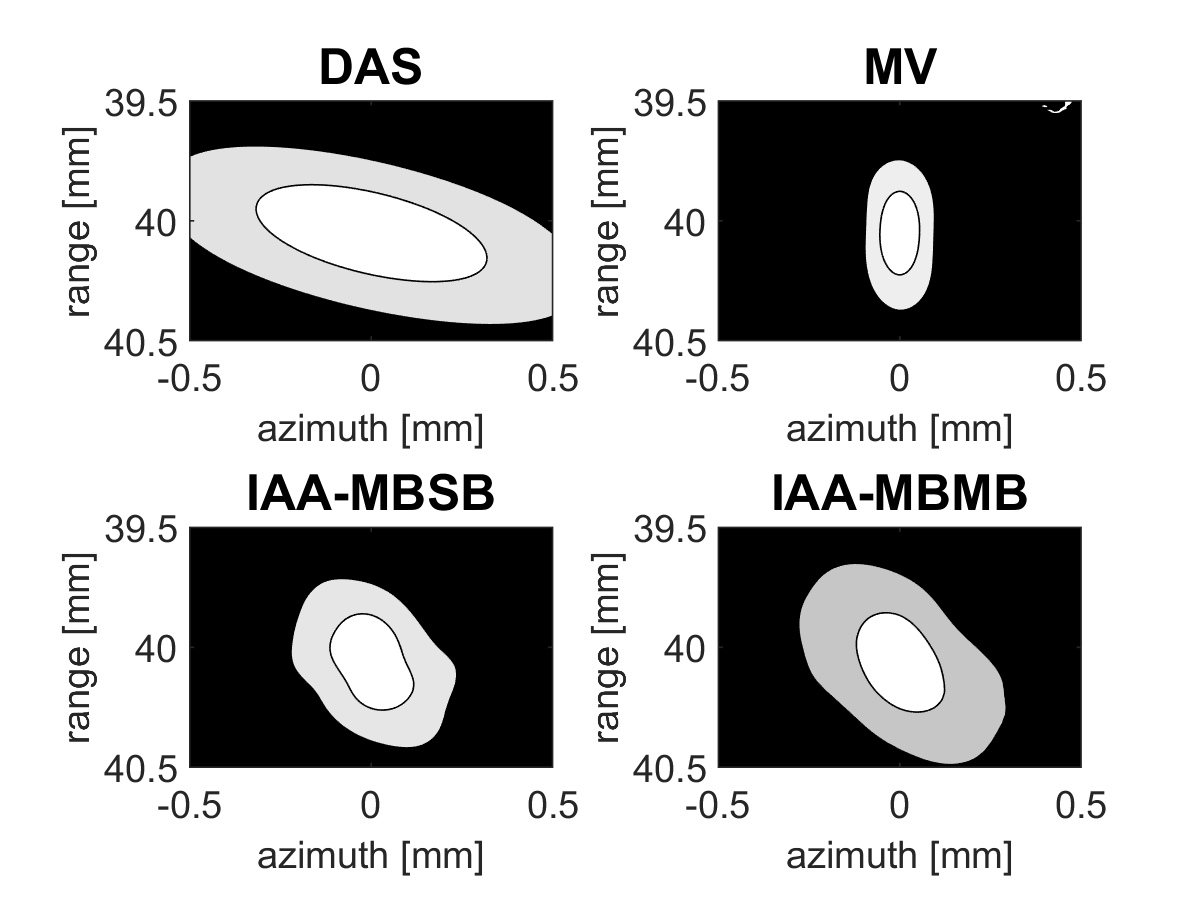
\includegraphics[width=\linewidth]{./images/results/2.1/motion_90_06.png}
        \caption{$\boldsymbol{v}_s = (0, 0.6)~m/s$.}
        \label{eq:vertical_away}
    \end{subfigure}
    \quad
    \begin{subfigure}[t]{0.48\linewidth}
        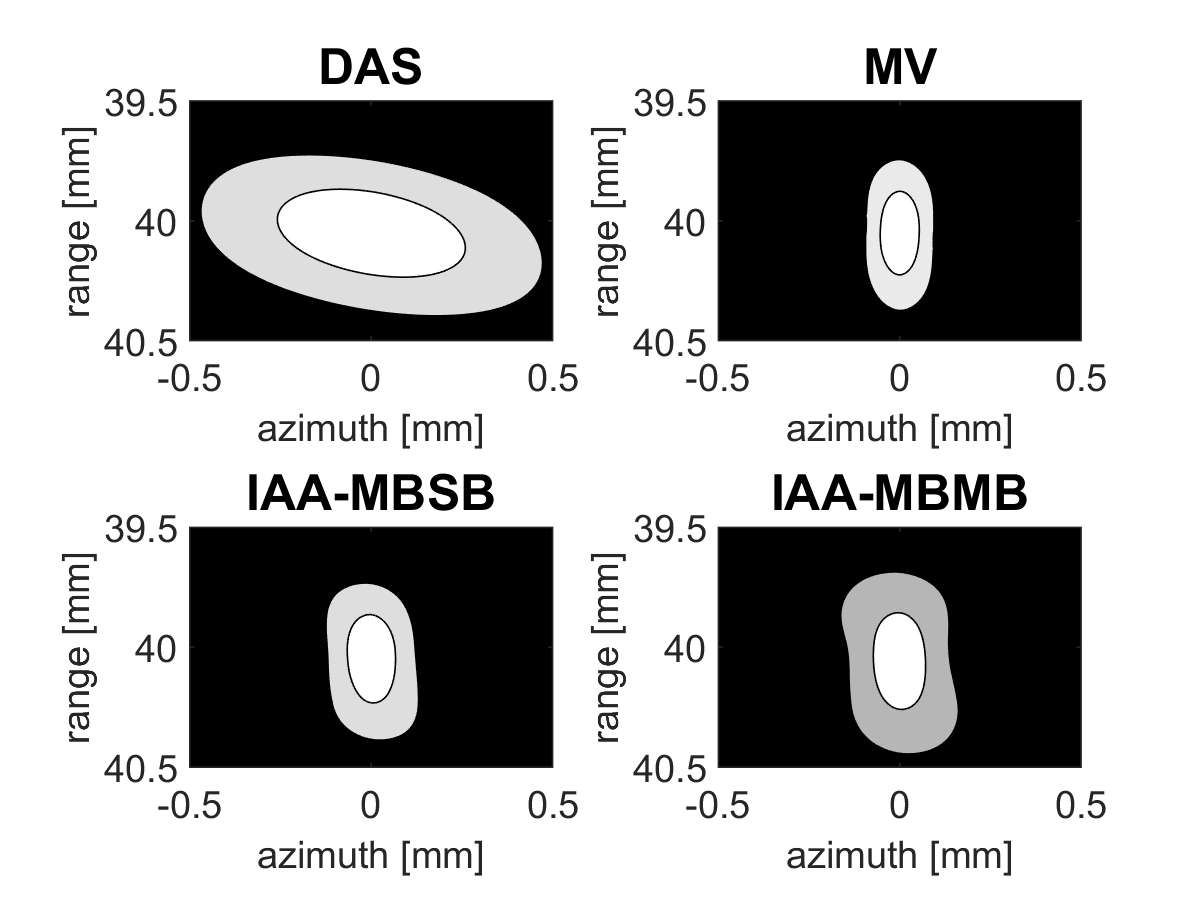
\includegraphics[width=\linewidth]{./images/results/2.1/motion_-45_-06.png}
        \caption{$\boldsymbol{v}_s = (-0.42, 0.42)~m/s$.}
    \end{subfigure}
    \quad
    \begin{subfigure}[t]{0.48\linewidth}
        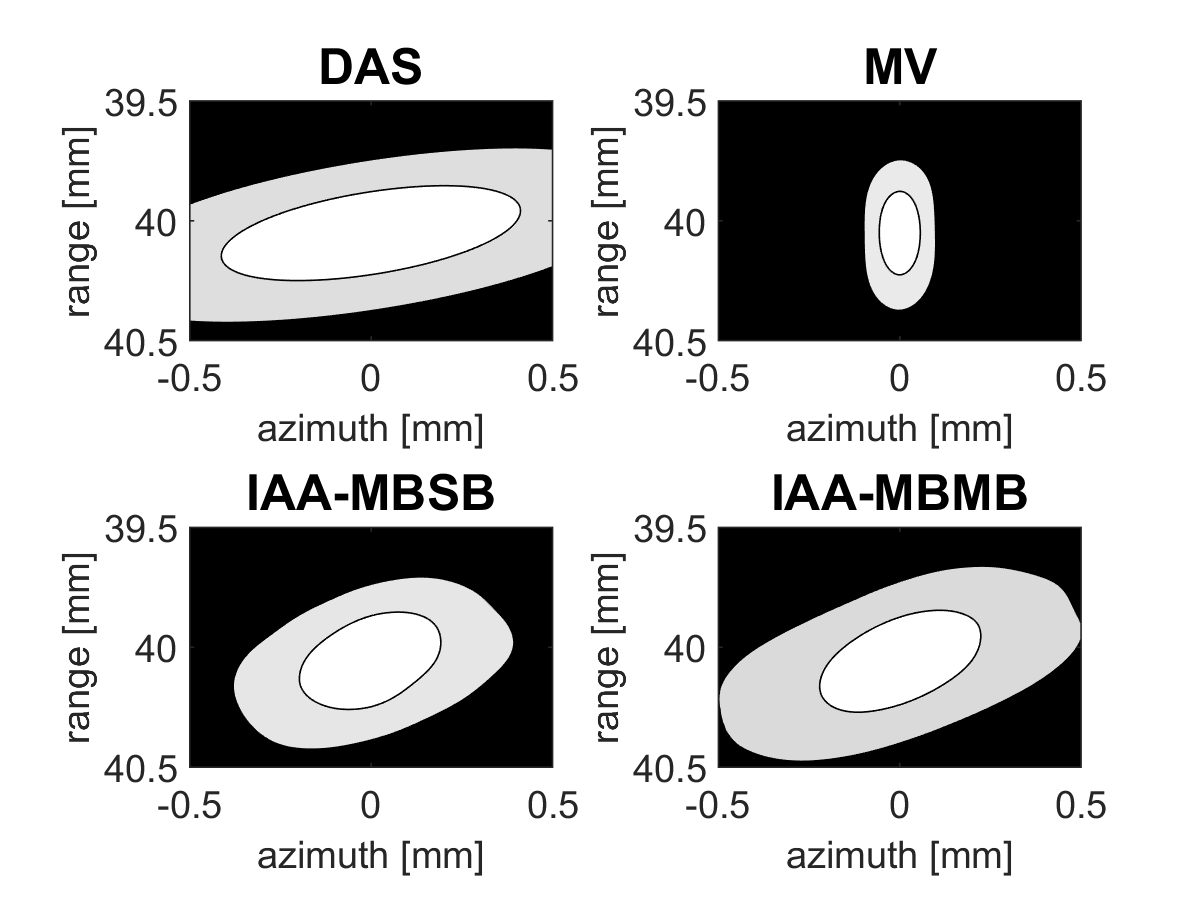
\includegraphics[width=\linewidth]{./images/results/2.1/motion_-45_06.png}
        \caption{$\boldsymbol{v}_s = (0.42, -0.42)~m/s$.}
    \end{subfigure}
    \quad
    \begin{subfigure}[t]{0.48\linewidth}
        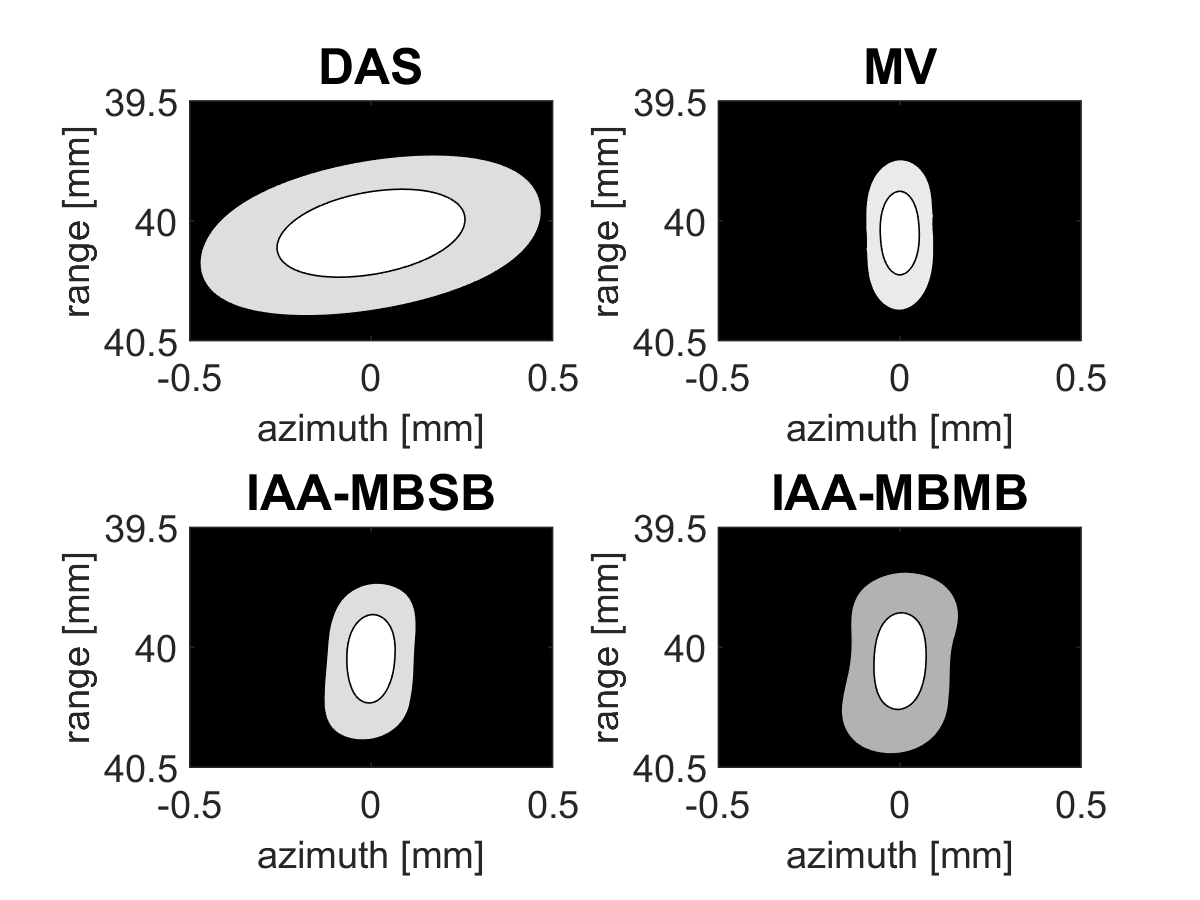
\includegraphics[width=\linewidth]{./images/results/2.1/motion_45_-06.png}
        \caption{$\boldsymbol{v}_s = (-0.42, -0.42)~m/s$.}
    \end{subfigure}
    \quad
    \begin{subfigure}[t]{0.48\linewidth}
        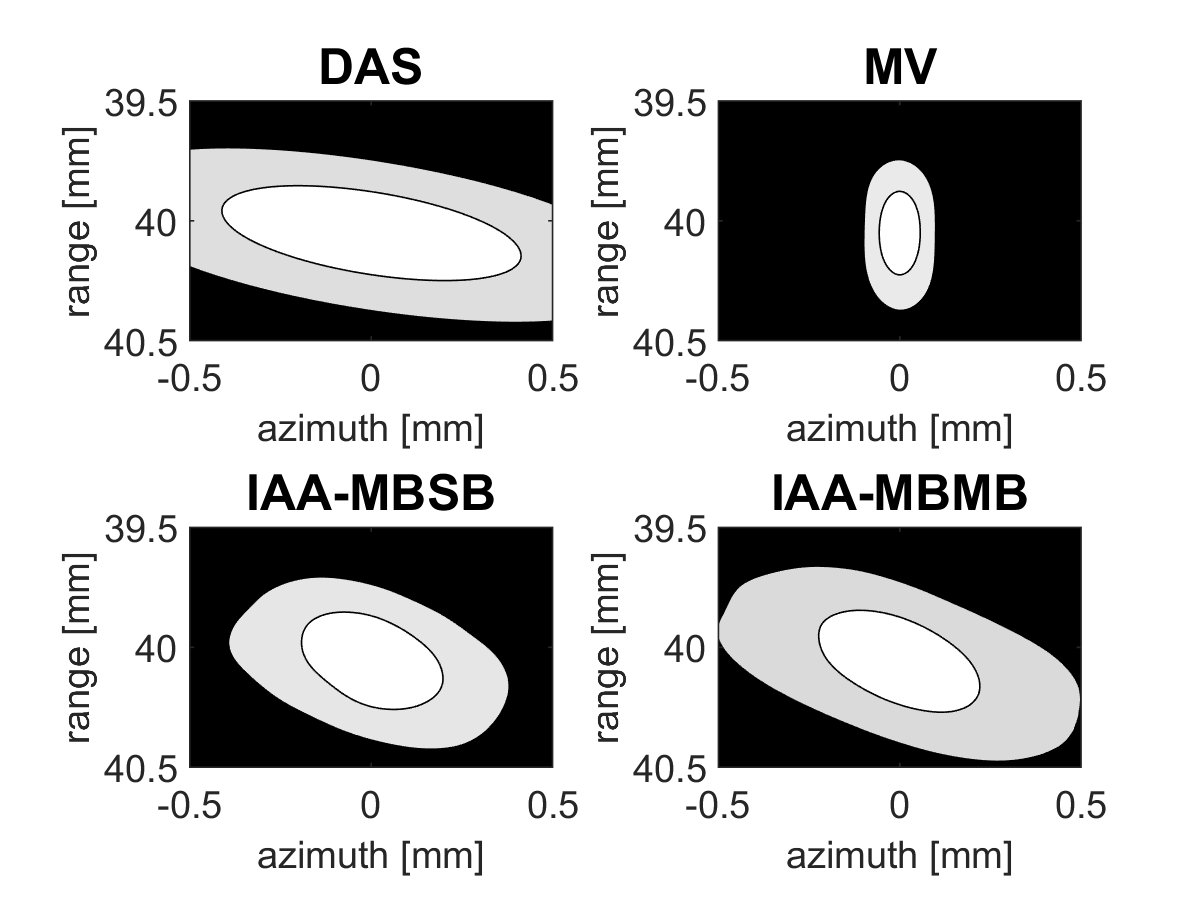
\includegraphics[width=\linewidth]{./images/results/2.1/motion_45_06.png}
        \caption{$\boldsymbol{v}_s = (0.42, 0.42)~m/s$.}
    \end{subfigure}
	\caption[A single scatterer point in various linear motions $\boldsymbol{v}_s$ with $|\boldsymbol{v}_s|=0.6~m/s$ in a noiseless medium.]{A single scatterer point in various linear motions $\boldsymbol{v}_s$ with $|\boldsymbol{v}_s|=0.6~m/s$ in a noiseless medium. Contour plot levels: max-100, max-10 and max-3 dB.}
	\label{fig:linear_motion}
\end{figure}


\clearpage
\subsection{Closely separated points in a noiseless medium}
\label{sec:twopoints_noiseless}
Section \ref{sec:spatial_smoothing} explored the issues with the presence of coherent signals in a recorded wavefield. Adaptive beamformers such as MV assume signals reflected by different scatterer points to be totally uncorrelated. Since active beamforming systems are by definition transmitting signals and recording their echoes from elements in the imaged medium, those echoes are by nature correlated.
This deviation from the model can induce apparent signal cancellation and result in lower SNR of the signals backscattered by the scatterer points in the imaged medium. The MV beamformer used in this thesis actively uses the spatial smoothing robustification method (Section \ref{sec:spatial_smoothing}) to decorrelate as much as possible the scatterer point echoes and reduce the signal cancellation effect.

The IAA approaches do not use spatial smoothing, since they are both based on the sparse signal representation and the multibeam covariance matrix estimate approaches.
As mentioned in Section \ref{sec:multibeam}, the multibeam approach can be used as an alternative method to spatial averaging to partially decorrelate spatially different signals.
Furthermore, due to the sparse signal representation, when fitting the recorded data into the covariance matrix model, the data from two closely-separated scatterer points does not match with any potential single point in the model.
For those reasons, spatial averaging is deemed not necessary for the IAA approaches.

Closely-separated scatterer points are a deviation from the expected model, not due to their proximity, since the model expects closely-separated points, but due to the high coherence of their respective backscattered signals.
The spatial averaging approach (Section \ref{sec:spatial_smoothing}) is used for the DAS and MV beamformers to decorrelate the backscattered signals. Since the length of the subarrays is typically taken as a user parameter, we can expect this approach to yield sub-optimal performances.
The IAA beamformers are able to decorrelate recorded signals without spatial averaging or required user parameter.
We therefore expect the IAA beamformers to globally yield more optimal corrections for signal coherence than the beamformers using spatial averaging.

However, we do not know how two closely-separated points in motion would affect the performances of the IAA beamformers.
We saw in Section \ref{sec:single_noiseless} that motion of a single scatterer point may result in shape distortion and resolution loss.
But the presence of motion with coherent signals might become too much of a deviation from the expected model for the IAA beamformers to correctly handle it.

In this section as well as the previous one, all beamformed images are considered to be built from $b_{tr} = 65$ transmit beams and $b_{re} = 3 \cdot 65 = 195$ receive beams by simulating perfect parallel receive beamforming. The beamformed images are also displayed as contour plots in order to outline the apparent shape of the scatterer points.
As defined in Section \ref{sec:aperture_smoothing}, two points are considered \textit{resolved} only if the minima between their peaks is of lower or equal amplitude than the lowest peak gain minus $3~$dB.
In the contour plots, the scatterer points are resolved only if their shape, delimited by the white colored layer, do not intersect.

Let us first start with static scatterer points. Two scatterer points $s_1$ and $s_2$ are simulated in a noiseless medium at $40~$mm range and respectively 0 and $0.75~$mm azimuth (or 0 and $1.07^\circ$).
With $b_{tr} = 65$, the distance between two transmit beams at $40~$mm range is $0.375~$mm. The scatterer points are therefore both located on a transmit beam trajectory and are separated by a transmit beam exactly in between them.
Since both points are static and on a transmit beam trajectory, they are not subject to scalloping loss.
The resulting beamformed images are displayed in Figure \ref{fig:two_points_static}.
In this case, none of the beamformers are able to resolve the two scatterer points, although the MV beamformer is very close to achieving it. The two points are spatially too correlated, or in other words too close to each other, for the beamformers to resolve them.

Before adding motion into the imaged scene, it is worth having a short reflection on the image acquisition sequence. In this thesis, an image is formed by sequentially transmitting and recording beams with their focus point shifted from negative azimuth to positive azimuth, or in other words, towards positive X (Figure \ref{fig:velocities}). Imagining that a scatterer point $s_1$ located at position $(x_1, y_1)$ is illuminated at time $t_1$, then any point $s_2$ located at position $(x_2, y_2)$, such that $x_2 > x_1$ is illuminated at time $t_2 \geq t_1$. If the scatterer points are not illuminated by the same transmit beam, then $t_2 > t_1$.
Let the true distance between $s_1$ and $s_2$ be $\delta x = x_2 - x1$ and the distance perceived by the beamformer be $\delta x_{BF}$.
Let us further assume that both $s_1$ and $s_2$ are moving at the same lateral velocity $v_x$.
Then the true distance $\delta x$ is constant regardless of $v_x$, but the perceived distance $\delta x_{BF}$ can vary depending on $\delta x$, $v_x$ and $\delta_t = t_2 - t_1$.
Based on those reflections, one could predict that lateral motion $v_x > 0$ may help to resolve closely separated scatterer points, since their apparent relative distance $\delta x_{BF}$ might increase. At the opposite, a lateral motion $v_x < 0$ may make it harder to resolve $s_1$ and $s_2$. 


\begin{figure}[ht]
    \centering
    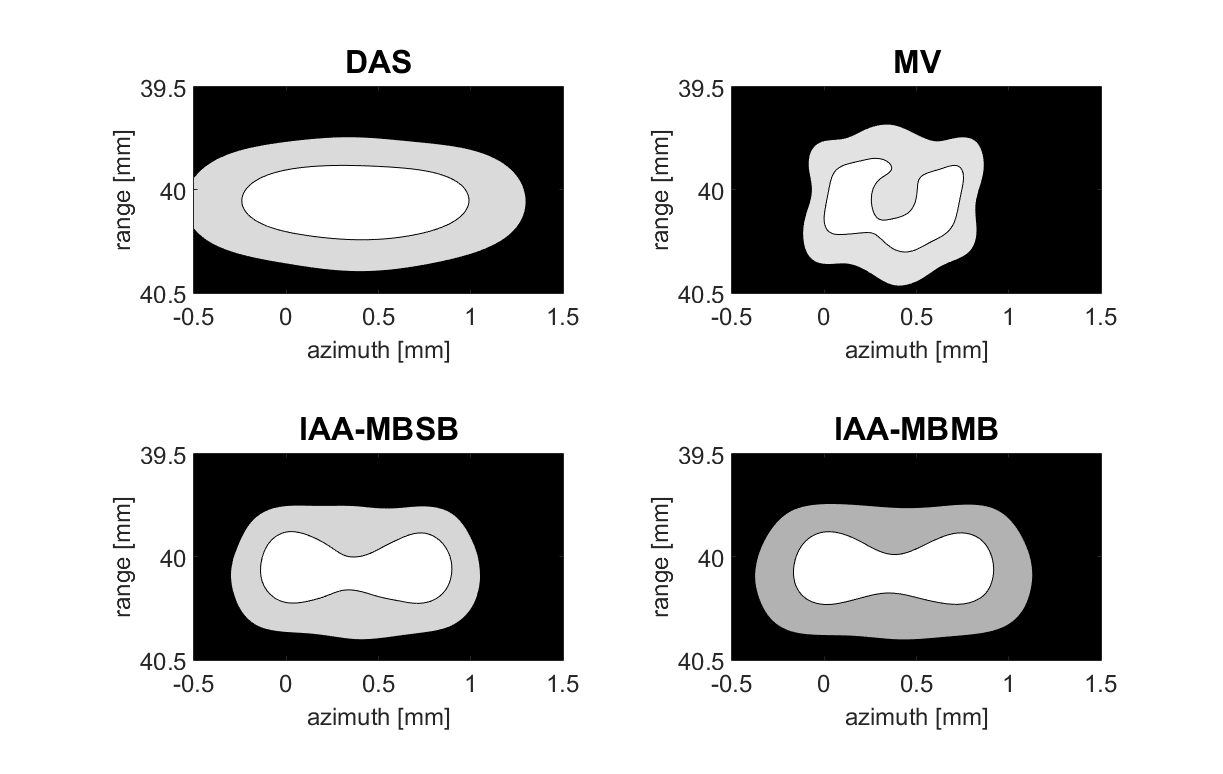
\includegraphics[width=\linewidth]{./images/results/2.2/motion_0_0.png}
    \caption[Contour plot of beamformed image with two closely-separated scatterer points in a noiseless medium.]{Contour plot of beamformed image with two closely-separated scatterer points in a noiseless medium. Color levels are: max-100, max-10 and max-3 dB.}
    \label{fig:two_points_static}
\end{figure}

Moving past static scatter points, the experiments of Section \ref{sec:single_noiseless} are reproduced with the following scenario.  Different images are simulated with the scatterer points moving in different directions at $0.6~$m/s in a noiseless medium.
In Section \ref{sec:single_noiseless}, the scatterer point was guaranteed to hit the center beam regardless of its velocity. In this section, this guarantee still holds for $s_1$, but not for $s_2$. If $s_2$ has a higher lateral velocity $v_x$ than that of the image acquisition, $v_{tr}$ as defined in Equation (\ref{eq:vtr}), it may even exit the image sector before being illuminated and would then not be detected. In our experiments, the number of transmit beams is set to $b_{tr} = 65$, which means that the image acquisition lateral velocity at $40~$mm range, defined in Equation (\ref{eq:vtr}), is $v_{tr} = 1500 \cdot 40 \cdot 10^{-3} / \lfloor b_{tr} / 2 \rfloor = 60 / 32 = 1.875~$m/s. Since the scatterer points lateral velocity $v_x \leq 0.6~$m/s, both points are guaranteed to be illuminated.
However, since $s_2$ is not guaranteed to perfectly hit a transmit beam trajectory, scalloping loss can occur. With $b_{re} = 195$ receive beams and perfect MLA, the scalloping loss is kept below the visibility threshold ($1~$dB) for the DAS, IAA-MBSB and IAA-MBMB beamformers. The effects of scalloping loss might be visible in the MV beamformed images.

The beamformed images resulting from this experiment are displayed in Figure \ref{fig:linear_motion_double} as contour plots similar to those of Figure \ref{fig:linear_motion}.
It may seem logical that introducing motion $v_x < 0$, opposite to the image acquisition direction, can add difficulties to resolve the two points, since their apparent distance $\delta x_{BF}$ decreases with $v_x$. One could then hope that the inverse is true as well, with $v_x > 0$ inducing an increased apparent distance and therefore increased chance of resolving $s_1$ and $s_2$. 
These assumptions seem to hold for the MV beamformer, but not for the IAA approaches. This can be explained by the fact that our MV beamformer is based on the single-beam covariance matrix estimation approach, whereas the IAA beamformers are based on the multibeam covariance matrix estimation (Section \ref{sec:multibeam}).
For single-beam beamformers, let us assume that the scatterer points are located in the direction matching that of the nearest beam. This assumption is technically false and a simplification of reality, but not that far from it for velocities $v_x$ well under $v_{tr}$. The first scatterer point is then always paired with the array's center beam ($\theta = 0$). If $s_2$ is paired with beam $n$, where $n=0$ is the center transmit beam, then its apparent distance to $s_1$ is $n \cdot d_B$. Lateral motion may then affect which beam $s_2$ is paired with and thus influence on the points' apparent distance.
This tendency is also true for the DAS beamformer, since it is also a single-beam beamformer. However, due to its poor resolution capacity, the DAS is not able to resolve the two scatterer points in any of the scenes of Figure \ref{fig:linear_motion_double}.

For multibeam beamformers, each beamformed image cell is built from multiple beams, so the scatterer points can not be paired with a single beam. 
If the scatterer point are moving, the beams hold different information about their location. As seen in Section \ref{sec:single_noiseless}, the more $v_x$ converges towards $v_{tr}$, the more beams are likely to illuminate the scatterer point. This divergence in the scatterer points apparent location can result in loss of resolvability.
For velocities in opposite direction ($v_x < 0$), fewer beams contain information about the same scatterer point, which means that the data is more likely to correspond to the expected model of static scatterer points.
Note that extreme velocities ($v_x < -1.2~$m/s) may cause mismatch with the expected model, since a point detected by a beam might not be detected by the neighboring beams, which might confuse the beamformer (Figure \ref{fig:width_vs_velocity_ext_neg}).

The multibeam beamformers are therefore more sensitive to positive lateral motion ($v_x > 0$) than the single-beam ones, but more robust to negative lateral motion ($v_x < 0$), at least to some extent.
The resolvability performances of the IAA approaches are, for $-0.6 \leq \boldsymbol{v}_s \leq 0.6~$m/s, at best better than MV and at worst similar to DAS.
The vertical component $v_y$ is less of a disturbance to the resolvability of the points than $v_x$. In fact, any vertical velocity, negative or positive, helps to differentiate the two points.
Figure \ref{fig:linear_motion_double} shows the same confusion of dilation direction than Figure \ref{fig:linear_motion}, where the direction of dilation $\boldsymbol{d}_s$ does not always point in the same direction as the scatterer point velocity vector $\boldsymbol{v}_s$.

\begin{figure}[ht]
    \centering
    \begin{subfigure}[t]{0.48\linewidth}
        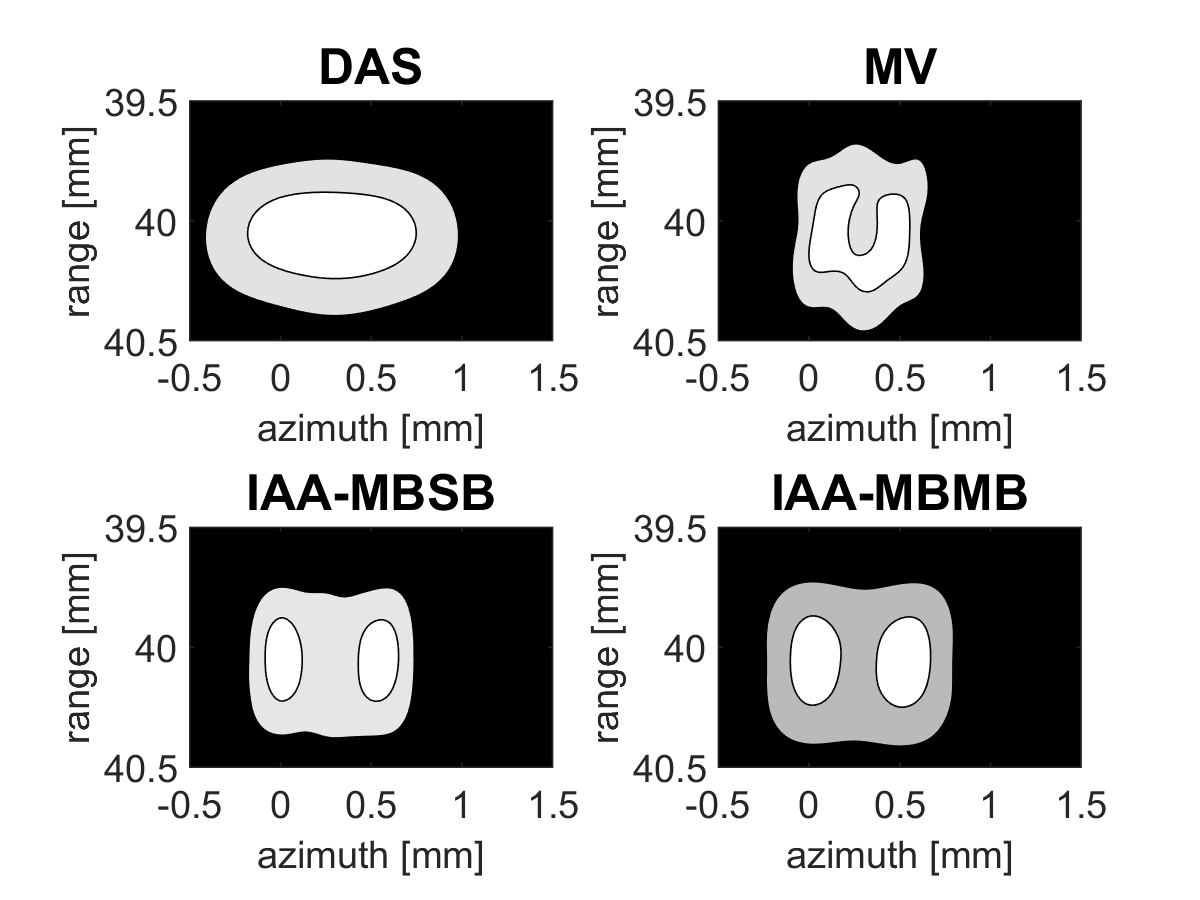
\includegraphics[width=\linewidth]{./images/results/2.2/motion_0_-06.png}
        \caption{$\boldsymbol{v}_s = (-0.6, 0)~$m/s.}
    \end{subfigure}
    \quad
    \begin{subfigure}[t]{0.48\linewidth}
        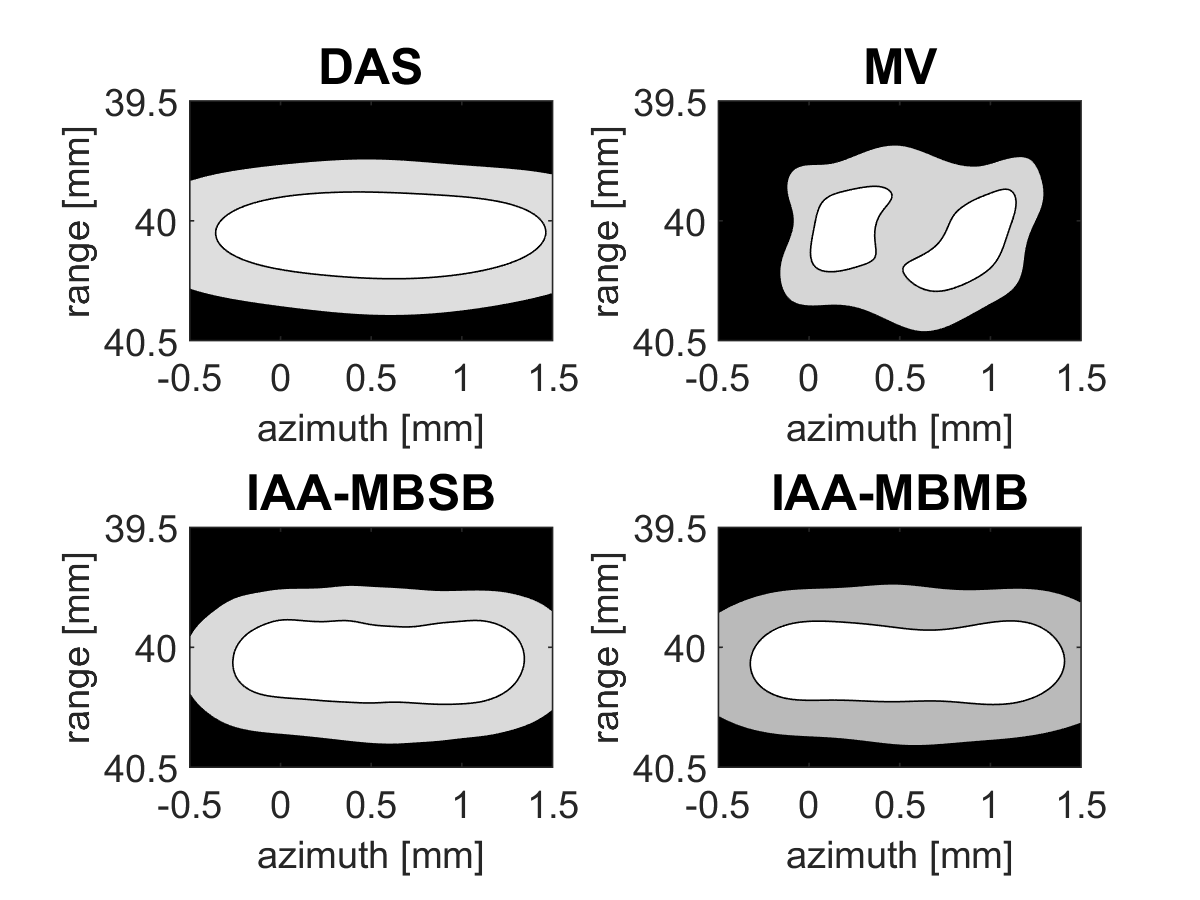
\includegraphics[width=\linewidth]{./images/results/2.2/motion_0_06.png}
        \caption{$\boldsymbol{v}_s = (0.6, 0)~$m/s.}
        \label{fig:double_lateral}
    \end{subfigure}
    \quad
    \begin{subfigure}[t]{0.48\linewidth}
        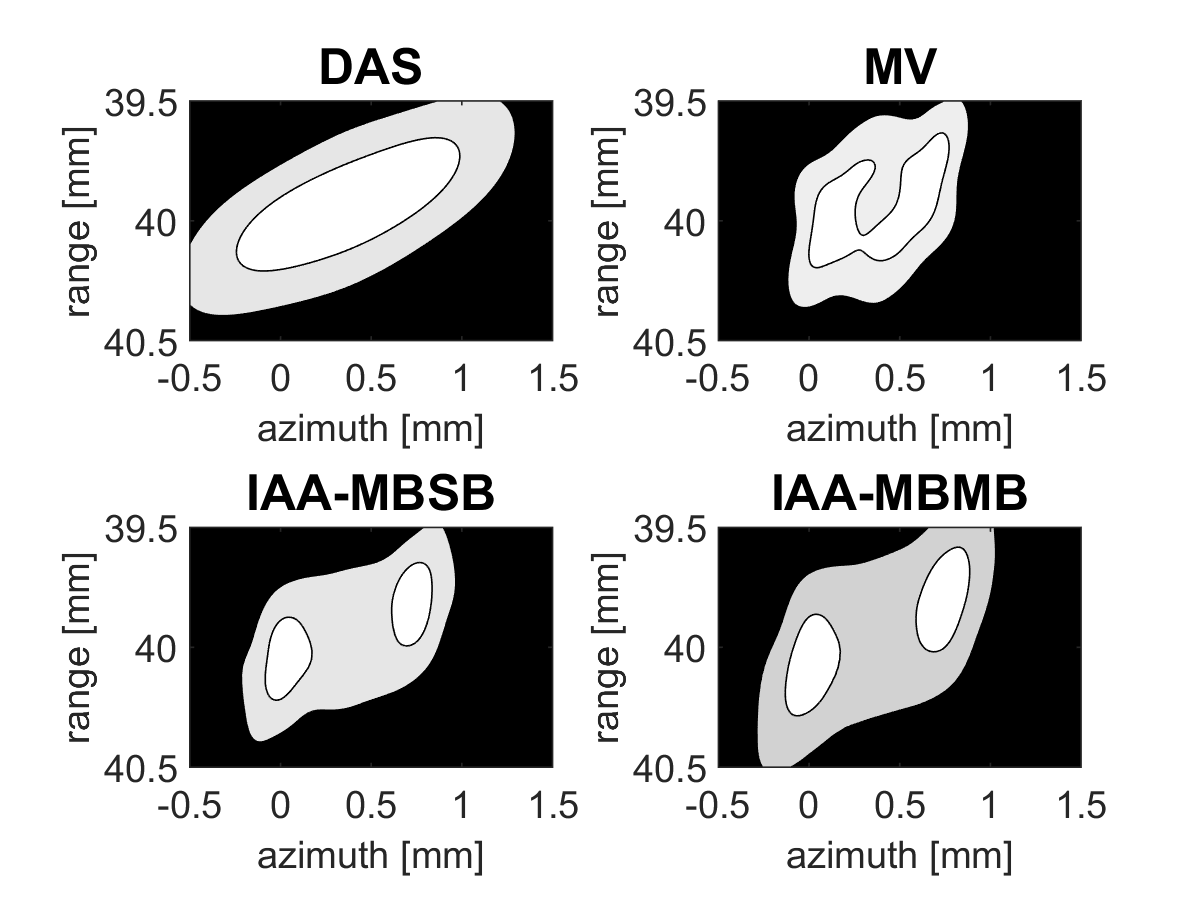
\includegraphics[width=\linewidth]{./images/results/2.2/motion_90_-06.png}
        \caption{$\boldsymbol{v}_s = (0, -0.6)~$m/s.}
    \end{subfigure}
    \quad
    \begin{subfigure}[t]{0.48\linewidth}
        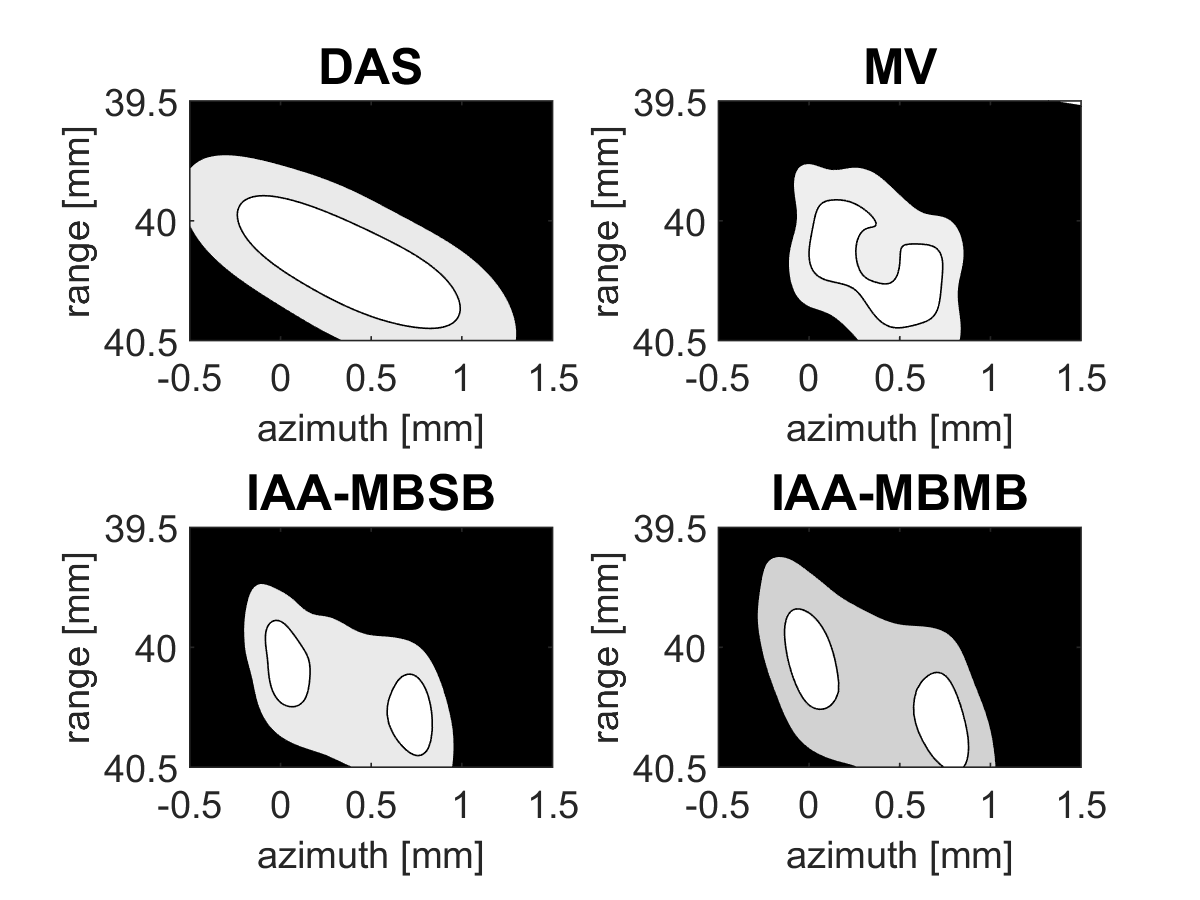
\includegraphics[width=\linewidth]{./images/results/2.2/motion_90_06.png}
        \caption{$\boldsymbol{v}_s = (0, 0.6)~$m/s.}
    \end{subfigure}
    \quad
    \begin{subfigure}[t]{0.48\linewidth}
        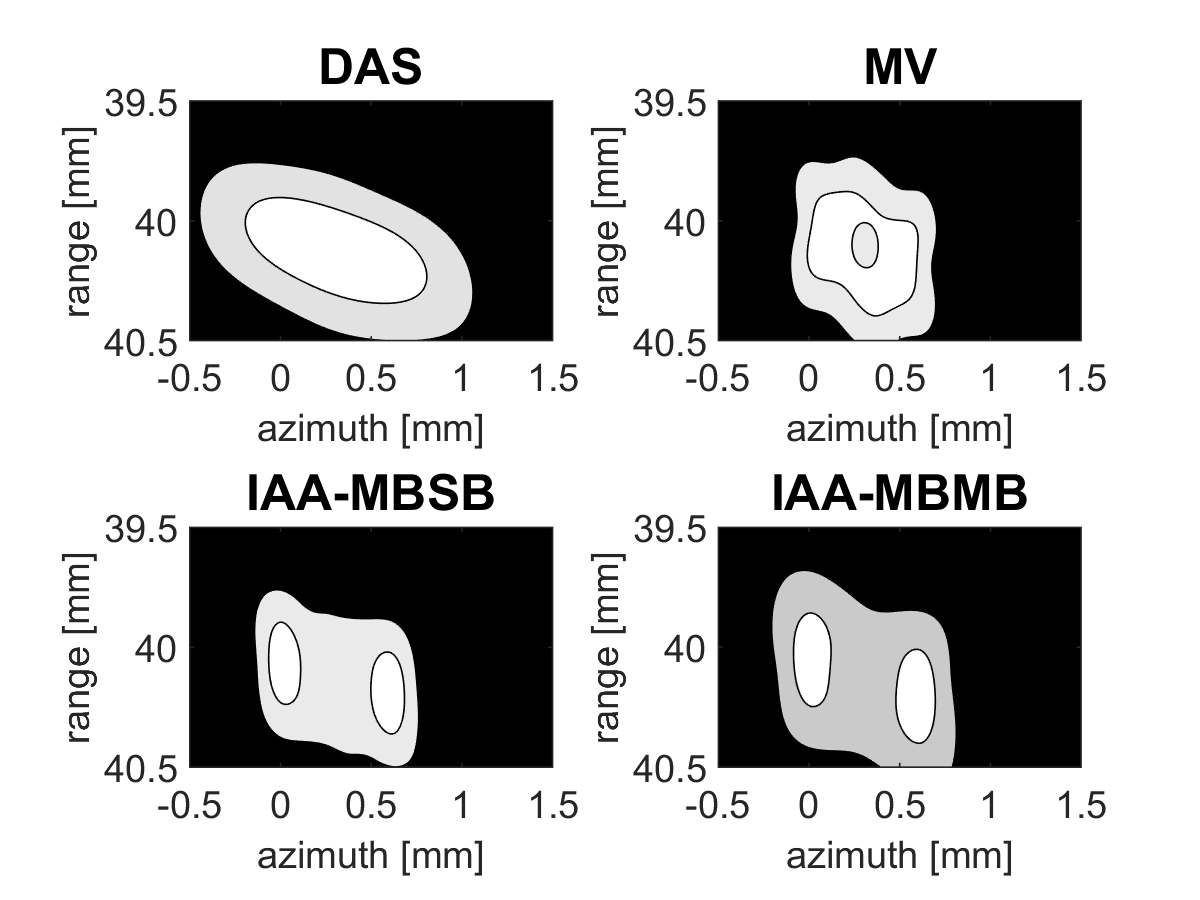
\includegraphics[width=\linewidth]{./images/results/2.2/motion_-45_-06.png}
        \caption{$\boldsymbol{v}_s = (-0.42, 0.42)~$m/s.}
    \end{subfigure}
    \quad
    \begin{subfigure}[t]{0.48\linewidth}
        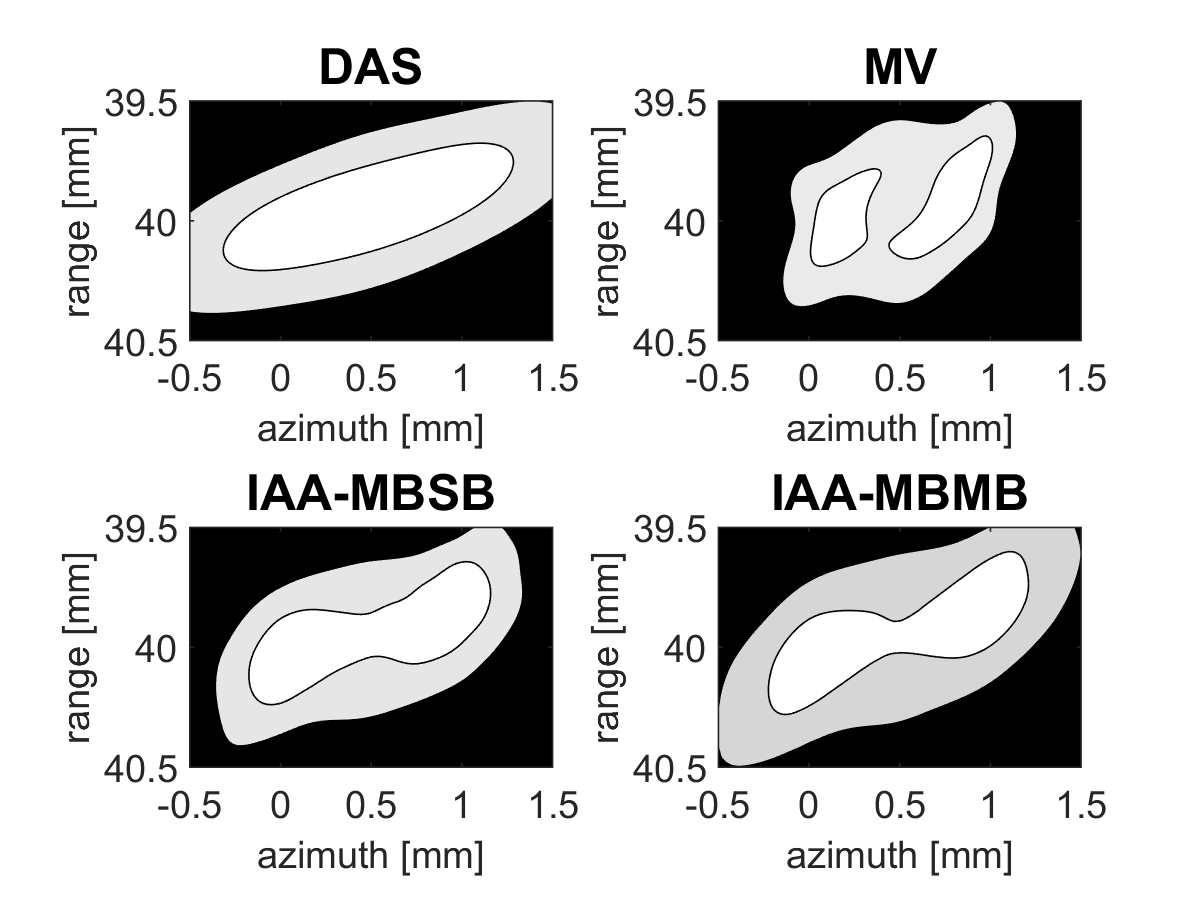
\includegraphics[width=\linewidth]{./images/results/2.2/motion_-45_06.png}
        \caption{$\boldsymbol{v}_s = (0.42, -0.42)~$m/s.}
    \end{subfigure}
    \quad
    \begin{subfigure}[t]{0.48\linewidth}
        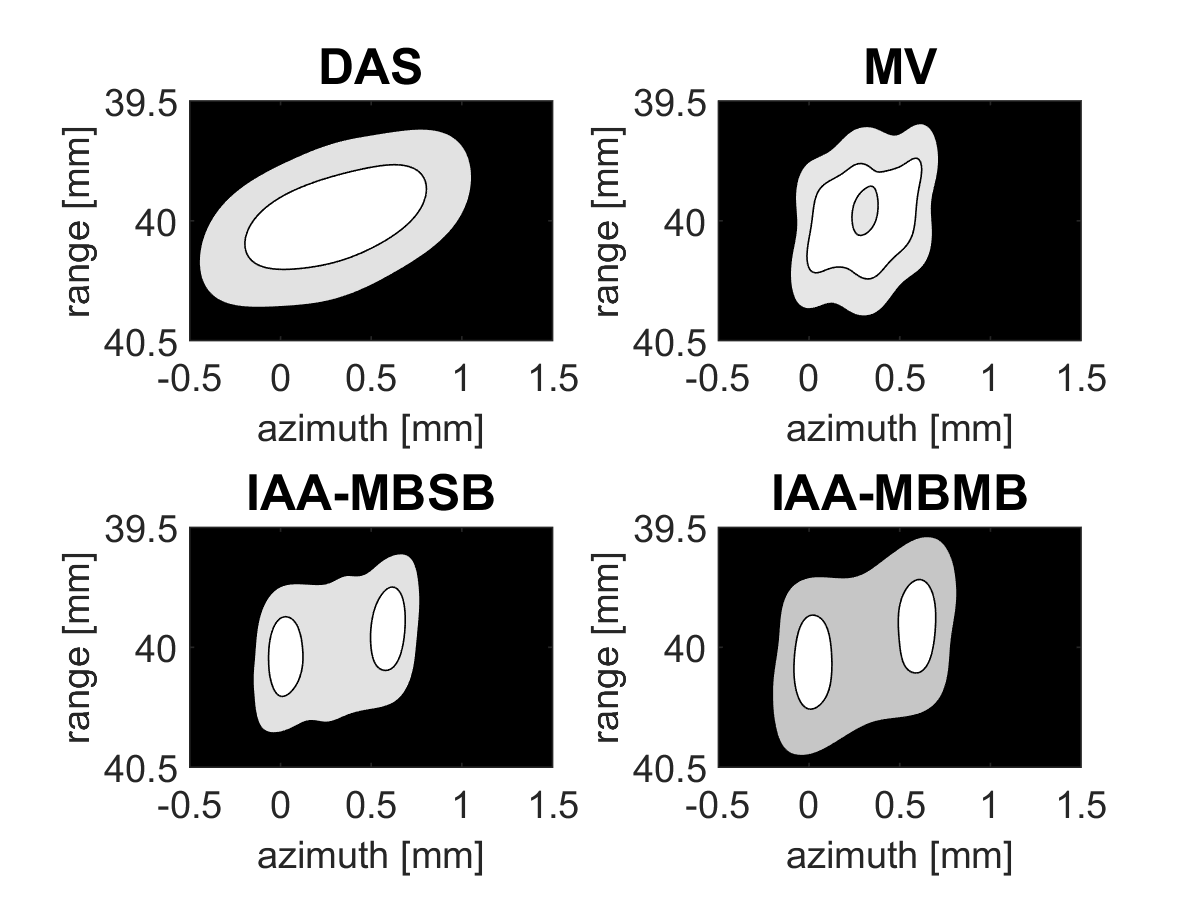
\includegraphics[width=\linewidth]{./images/results/2.2/motion_45_-06.png}
        \caption{$\boldsymbol{v}_s = (-0.42, -0.42)~$m/s.}
    \end{subfigure}
    \quad
    \begin{subfigure}[t]{0.48\linewidth}
        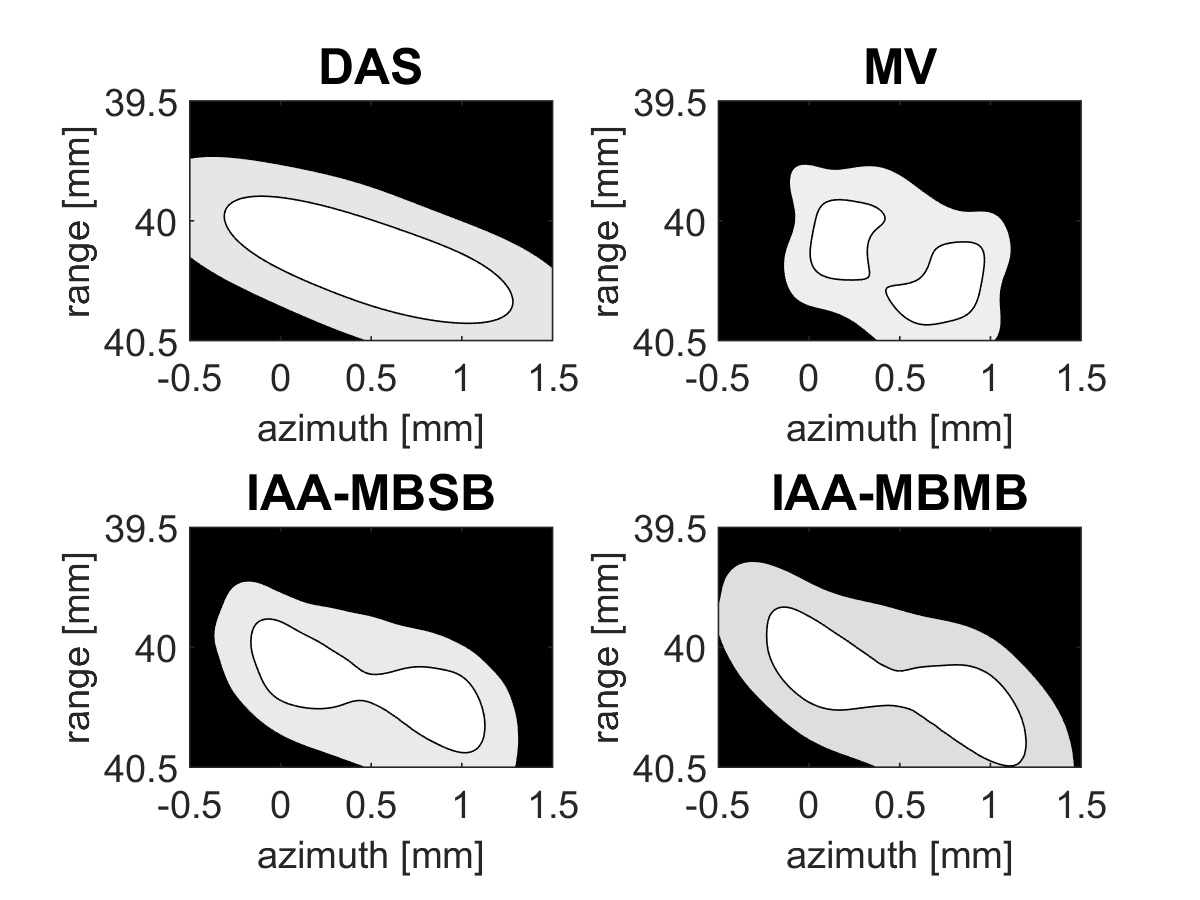
\includegraphics[width=\linewidth]{./images/results/2.2/motion_45_06.png}
        \caption{$\boldsymbol{v}_s = (0.42, 0.42)~$m/s.}
    \end{subfigure}
	\caption[Two scatterer points, initially $0.75~$mm apart, in various linear motions $\boldsymbol{v}_s$ with $|\boldsymbol{v}_s|=0.6~$m/s in a noiseless medium.]{Two scatterer points, initially $0.75~$mm apart, in various linear motions $\boldsymbol{v}_s$ with $|\boldsymbol{v}_s|=0.6~$m/s in a noiseless medium. Contour plot levels: max-100, max-10 and max-3 dB.}
	\label{fig:linear_motion_double}
\end{figure}
